	%%%%%%%%%%%%%%%%%%%%%%%%%%%%%%%%%%%%%%%%%%%%%%%%%%%%%%%%%%%%%%%%%%%%%%%%%%%%%%%
%                       CARREGA DE LA CLASSE DE DOCUMENT                      %
%                                                                             %
% Les opcions admissibles son:                                                %
%      12pt / 11pt            (cos dels tipus de lletra; no feu servir 10pt)  %
%                                                                             %
% catalan/spanish/english     (llengua principal del treball)                 %
%                                                                             % 
% french/italian/german...    (si necessiteu fer servir alguna altra llengua) %
%                                                                             %
% listoffigures               (El document inclou un Index de figures)        %
% listoftables                (El document inclou un Index de taules)         %
% listofquadres               (El document inclou un Index de quadres)        %
% listofalgorithms            (El document inclou un Index d'algorismes)      %
%                                                                             %
%%%%%%%%%%%%%%%%%%%%%%%%%%%%%%%%%%%%%%%%%%%%%%%%%%%%%%%%%%%%%%%%%%%%%%%%%%%%%%%

\documentclass[11pt,english,listoffigures,listoftables]{tfgetsinf}

%%%%%%%%%%%%%%%%%%%%%%%%%%%%%%%%%%%%%%%%%%%%%%%%%%%%%%%%%%%%%%%%%%%%%%%%%%%%%%%
%                     CODIFICACIO DEL FITXER FONT                             %
%                                                                             %
%    windows fa servir normalment 'ansinew'                                   %
%    amb linux es possible que siga 'latin1' o 'latin9'                       %
%    Pero el mes recomanable es fer servir utf8 (unicode 8)                   %
%                                          (si el vostre editor ho permet)    % 
%%%%%%%%%%%%%%%%%%%%%%%%%%%%%%%%%%%%%%%%%%%%%%%%%%%%%%%%%%%%%%%%%%%%%%%%%%%%%%%

\usepackage[utf8]{inputenc} 
\usepackage{amsmath}
%\usepackage[demo]{graphicx}
\usepackage{subfig}
\usepackage{pdfpages}
%\usepackage{ods_etsinf}

%%%%%%%%%%%%%%%%%%%%%%%%%%%%%%%%%%%%%%%%%%%%%%%%%%%%%%%%%%%%%%%%%%%%%%%%%%%%%%%
%                        ALTRES PAQUETS I DEFINICIONS                         %
%                                                                             %
% Carregueu aci els paquets que necessiteu i declareu les comandes i entorns  %
%                                          (aquesta seccio pot ser buida)     %
%%%%%%%%%%%%%%%%%%%%%%%%%%%%%%%%%%%%%%%%%%%%%%%%%%%%%%%%%%%%%%%%%%%%%%%%%%%%%%%

\newcommand{\vect}[1]{\mathbf{#1}}



%%%%%%%%%%%%%%%%%%%%%%%%%%%%%%%%%%%%%%%%%%%%%%%%%%%%%%%%%%%%%%%%%%%%%%%%%%%%%%%
%                        DADES DEL TREBALL                                    %
%                                                                             %
% titol, alumne, tutor i curs academic                                        %
%%%%%%%%%%%%%%%%%%%%%%%%%%%%%%%%%%%%%%%%%%%%%%%%%%%%%%%%%%%%%%%%%%%%%%%%%%%%%%%

\title{Streaming neural machine translation systems from English into European languages}
\author{Guillem Calabuig Domenech}
\tutor{Jorge Civera Saiz \\ Javier Iranzo Sánchez}
\curs{2021-2022}

%%%%%%%%%%%%%%%%%%%%%%%%%%%%%%%%%%%%%%%%%%%%%%%%%%%%%%%%%%%%%%%%%%%%%%%%%%%%%%%
%                     PARAULES CLAU/PALABRAS CLAVE/KEY WORDS                  %
%                                                                             %
% Independentment de la llengua del treball, s'hi han d'incloure              %
% les paraules clau i el resum en els tres idiomes                            %
%%%%%%%%%%%%%%%%%%%%%%%%%%%%%%%%%%%%%%%%%%%%%%%%%%%%%%%%%%%%%%%%%%%%%%%%%%%%%%%

\keywords{Traducció automàtica; traducció automàtica neuronal; traducció automàtica en streaming}
         {Traducción automática; traducción automática neuronal; traducción automática en streaming}
         {Machine Translation; Neural Machine Translation; Streaming Machine Translation}

%%%%%%%%%%%%%%%%%%%%%%%%%%%%%%%%%%%%%%%%%%%%%%%%%%%%%%%%%%%%%%%%%%%%%%%%%%%%%%%
%                              INICI DEL DOCUMENT                             %
%%%%%%%%%%%%%%%%%%%%%%%%%%%%%%%%%%%%%%%%%%%%%%%%%%%%%%%%%%%%%%%%%%%%%%%%%%%%%%%

\begin{document}

%%%%%%%%%%%%%%%%%%%%%%%%%%%%%%%%%%%%%%%%%%%%%%%%%%%%%%%%%%%%%%%%%%%%%%%%%%%%%%%
%              IESUMS DEL TFG EN VALENCIA, CASTELLA I ANGLES                  %
%%%%%%%%%%%%%%%%%%%%%%%%%%%%%%%%%%%%%%%%%%%%%%%%%%%%%%%%%%%%%%%%%%%%%%%%%%%%%%%

\begin{abstract}
La traducció automàtica (MT, de l’anglès Machine Translation) és una dels àrees més
actives dins de la intel·ligència artificial, particularment en el camp de l’aprenentatge
automàtic. Recentment, aquesta àrea ha sigut el focus d’atenció per part d’importants
figures tecnològiques com Google, Facebook, Microsoft, etc. a causa de les millores de
rendiment obtingudes per aquesta tecnologia gràcies a la incorporació de xarxes neuronals artificials. Un dels principals motius que explica està atenció és l’enorme creixement
de plataformes de difusió de continguts audiovisuals en streaming (per exemple YouTube
i Twitch) i vídeo-conferencia (per exemple Zoom i Webex). En aquest context, un aspecte
molt important és l’adaptació de tècniques i models convencionals per al seu ús en streaming, això és, per a un flux d’entrada a traduir constant i eixida ajustada per davall d’un
temps de resposta (latència) donat. En aquest treball es proposa estudiar i implementar
models avançats de MT neuronal en streaming, de l'anglès a llengües europees. Per a
això, es farà ús de dades, tecnologia i experiència del grup MLLP del VRAIN, adquirits
en el marc de projectes d’investigació i transferència tecnològica desenvolupats en els
últims anys.
\end{abstract}
\begin{abstract}[spanish]
La traducción automática (MT, del inglés Machine Translation) es una de les áreas más activas dentro de la inteligencia artificial, particularmente en el campo del aprendizaje automático. Recientemente, esta área ha sido el foco de atención por parte de importantes figuras tecnológicas como Google, Facebook, Microsoft, etc. debido a las mejoras de rendimiento obtenidas por esta tecnología gracias a la incorporación de redes neuronales artificiales. Uno de los principales motivos que explica está atención es el enorme crecimiento de plataformas de difusión de contenidos audiovisuales en streaming (por ejemplo YouTube y Twitch) y video-conferencia (por ejemplo Zoom y Webex). En este contexto, un aspecto muy importante es la adaptación de técnicas y modelos convencionales para su uso en streaming, esto es, para un flujo de entrada a traducir constante y salida ajustada por debajo de un tiempo de respuesta (latencia) dado. En este trabajo se propone estudiar e implementar modelos avanzados de MT neuronal en streaming, de inglés a lenguas europeas. Para ello, se hará uso de datos, tecnología y experiencia del grupo MLLP del VRAIN, adquiridos en el marco de proyectos de investigación y transferencia tecnológica desarrollados en los últimos años.
\end{abstract}
\begin{abstract}[english]
Machine translation is one of the most active areas within Artificial Intelligence, particularly in the field of Machine Learning. Recently, this area has been the focus of attention by major technology figures such as Google, Facebook, Microsoft, etc. due to the performance improvements obtained by this technology thanks to the incorporation of artificial neural networks. One of the main reasons for this attention is the enormous growth of streaming audiovisual content platforms (for example, YouTube and Twitch) and video-conferencing (for example, Zoom and Webex). In this context, a very important aspect is the adaptation of conventional techniques and models to be used in the streaming scenario, that is, the translation of a constant input flow under response time (latency) constraints. In this work it is proposed to study and implement advanced models of neural MT in streaming, from English into European languages. For this, data, technology and experience of the VRAIN MLLP group, acquired in the framework of research and technology transfer projects developed in recent years, will be used.
\end{abstract}

%%%%%%%%%%%%%%%%%%%%%%%%%%%%%%%%%%%%%%%%%%%%%%%%%%%%%%%%%%%%%%%%%%%%%%%%%%%%%%%
%                              CONTINGUT DEL TREBALL                          %
%%%%%%%%%%%%%%%%%%%%%%%%%%%%%%%%%%%%%%%%%%%%%%%%%%%%%%%%%%%%%%%%%%%%%%%%%%%%%%%

\mainmatter

%%%%%%%%%%%%%%%%%%%%%%%%%%%%%%%%%%%%%%%%%%%%%%%%%%%%%%%%%%%%%%%%%%%%%%%%%%%%%%%
%                                  INTRODUCCIO                                %
%%%%%%%%%%%%%%%%%%%%%%%%%%%%%%%%%%%%%%%%%%%%%%%%%%%%%%%%%%%%%%%%%%%%%%%%%%%%%%%

\chapter{Introduction}\label{intro}

In this chapter we present the motivations, goals and theoretical backgrounds of our work. We present the foundations of machine learning (ML), machine translation (MT) as well as neural models and state of the art architectures for language processing tasks. In addition, we describe the framework in which our labour is developed and the structure of this document.

\section{Motivation}

Nowadays' high computational capacity and worlwide continuous research over the years has brought artificial intelligence to succeed in a wide range of formerly unexpected tasks, in addition to its presence in almost all areas of application: corporative, commercial, administrative, research, industrial, health, entertainment, media, etc. This can be observed from simple applications to complex problems such as protein folding prediction \cite{Jumper2021HighlyAP}, communication restorage for patients with lost speech \cite{Willett2020.07.01.183384}, rocket driving \cite{https://doi.org/10.48550/arxiv.2102.07109}, cancer prognosis \cite{doi:10.1177/117693510600200030}, image generation from written text \cite{https://doi.org/10.48550/arxiv.2204.06125}, etc. Regarding our area of research, automatic translation of languages is already a reality in our daily lives, while there are still limits to push, milestones to achieve and research paths to explore. We can now for free translate within instants any phrase that we want to express in another language, and even translate it from raw speech. Massive amounts of text are also translated everyday internally within companies' workflow as well as externally for products and services. Technology corporations such as Amazon\footnote{https://aws.amazon.com/translate/}, Meta\footnote{https://ai.facebook.com/blog/nllb-200-high-quality-machine-translation/} or Google\footnote{https://translate.google.com/} develop their own machine translation systems which are also available for public use.

Improving the quality of state of the art translation systems as well as pushing towards achieving competitive live real time machine translation saves big amounts of resources and matches a growing demand, as online conferences and streaming media become more and more common in today's society. In the case of institutions like the European Organization for Nuclear Research (CERN), there is need of tailored translation systems that fit their vocabulary in specific domains such as physics. These systems cannot be provided by large corporations, since they are focused on general-purpose systems, in addition to data protection and privacy concerns. There is a market niche for domain-adapted systems to be developed by mid-size institutions such as university research groups, which are able to fit more specific requirements. This is the case of the collaboration between the CERN and the Machine Learning and Language Processing (MLLP) group at UPV, where this work is contextualized as we explain in Section \ref{framework}.

\section{Goals}

We can summarize the main objectives of the present work as follows:
\begin{itemize}
    \item To understand the theoretical developments and technological advances have led nerual machine translation (NMT) to be the current state of the art.
    \item To learn and showcase the different components and processes involved in the development of NMT systems, as well as the importance of data and how it is compiled for these systems.
    \item To improve the offline NMT models for the English to French translation task that already exist in the MLLP research group.
    \item To explore, compare and apply different methods to adapt NMT systems to a specific domain in order to significantly improve the translation quality in in-domain evaluation tasks.
    \item To understand the challenges that exist in building streaming and real time NMT models, how they are evaluated, and construct a system for such task based on offline system results.
    \item To develop MT systems ready to be deployed and used in real scenarios for the English to French translation task.
\end{itemize}

\section{Machine Learning}\label{ml}

Artificial Inteligence is built upon the grounds of computers running instructions, as any other kind of instructions that they would run, but these in appearance resembling actions that are attributed to intelligence and in many occasions mimicking tasks done by humans.
 
The present work belongs to the branch of Artificial Intelligence called Machine Learning. In contrast to other branches, the intelligent behaviour of a system is achieved based mainly on the data that we make available to the system.

We could see the objective of a Machine Learning system as the task of offering correct answers to a certain set of questions. Let these questions be of any kind, whether a patient suffers from cancer or not, should the car turn left, right or stop, which is the next film that we should recommend a user to watch, etc. In the task that ensues us our systems will be trying to give proper answers to the question of what is a good translation of a sentence into another language.

A system initially gives answers that are very distant to what we consider correct, and as it processes the data that we have provided to it, its performance increases. Thus we say that the system has \textit{learnt} from the data.

In its basis a ML system is a computer program that materializes (in a big physical arena of transistors) a mathematical model, often a function, to which we give as argument our question and computes the answer depending on a set of \textit{weights}, operations and structure. These weights vary their values through an optimization process that depends on data, to which we refer as \textit{training}. Learning is thus the result of the system having found a set of values for the weights that make the model offer better answers to the problem presented.

In other words, referring to the definition of Machine Learning by Tom Mitchell \cite{BookTM}: 

"A computer program is said to learn from experience E with respect to some class of tasks T, and performance measure P, if its performance at tasks in T, as measured by P, improves with experience E"

A function is optimized from data \textit{E} to answer questions \textit{T} these being more or less correct according to \textit{P}.
A lot of engineering work, scientific research and experimentation is performed in order to discover better weight-keeping structures, model configurations and optimization processes that allow coming up with better weights (learning) that achieve better performance (more useful answers) to a specific task (question) from experience (data). 

\subsection{Supervised learning and classification}\label{sl}
Many problems or question-answering instances can be viewed as a \textit{classification} task, that falls into the branch of Machine Learning known as \textit{supervised learning}. In this scenario, data or experience to learn from comes as a pair (\textbf{x}, \textbf{c}), \textbf{x} being the object to be classified and \textbf{c} being the correct answer or \textit{class} to which \textbf{x} should be classified to.

We keep in mind that the usefulness of a system and the ultimate goal always comes in answering questions for which there is uncertainty, inputs \textbf{x} for which the right class \textbf{c} is not known. 
Output a correct classification to new samples of the task, that have not been involved during the training of the model.
We are referring here to performing \textit{inference}.

But the model will learn to improve the performance on this task from the knowledge that is present in well-answered question pairs, that is, correct solutions to instances of the same kind of problems.
%A model that generalizes, being able to offer a solution to a question for which the answer has not yet seen. 

The final objective is to construct a system where false answers are minimized. In other words, provide solutions to tasks \textit{T} so that performance \textit{P} is maximized, i.e. minimize the number of mistaken classifications. We can see a formalization of the problem in the following section describing one of the first theoretical classification models. 

\subsubsection{Bayes classifier}
According to the statistical decision theory, 
we can define $p_c(error | \vect{x})$ as the probability of sample \textbf{x} to be classified into an incorrect class c and $p(c | \vect{x})$, the probability of \textbf{x} to belong to class c
\begin{equation}
    p_c(error | \vect{x}) = 1 - p( \vect{c}= c | \vect{x})
\end{equation}
and pick the label that minimizes the error: 
\begin{equation}
    \min_{c \in C} p_c(error | \vect{x} ) = 1 - \max_{c \in C} p(c| \vect{x})
\end{equation}
\begin{equation}\label{cagmx}
    \vect{\hat{c}} = \arg \max_{c \in C} p(c| \vect{x})
\end{equation}
where $C$ is the set of possible class labels and $\vect{\hat{c}} $ the class decided by the system.
We refer to this as the minimum risk decision rule or Bayes classifier.

If the true distribution $p_c(c|\vect{x})$ was known for every \textbf{x}, we would have an optimal performance, an oracle, since \textbf{x} would always be classified into the most probable class, thus assignments of \textbf{x} to other classes would incur in more errors.

We could understand ML as a way where we are building a model that tries to approximate better the probabilities of $\vect{x}$ to be classified into class $\vect{c}$, using for such task the information that is available in the data supplied to our system. The use of the Bayes rule can be seen to derive an expression that is easier to approximate 
\begin{equation}\label{bayesxc}
    \arg \max_{c \in C} p(c| \vect{x}) =  \arg \max_{c \in C} \frac{p(\vect{x} | c) p(c)}{p(\vect{x})} = \arg \max_{c \in C} p(\vect{x} | c) p(c)
\end{equation}
where $p(\vect{x})$ is dropped since it is a constant term that does not modify the argument result of the optimization.

%\subsubsection{Iris dataset example}
%Consider the case where we had only 2 possible outcomes $c \in \{0,1\}$. Just 2 possible answers. Taking the \textbf{Iris dataset}\footnote{https://archive.ics.uci.edu/ml/datasets/iris} as an example, a question could be, given the petal length and petal width of this flower (as vector $\vect{x} \in  \mathbb{R}^2$), is it a virginica type flower or is not?
%
%We then could model this uncertainty under a Bernoulli distribution. The probability that the flower is virginica would be computed depending on the information of the petal, and a set of weights $\vect{w} \in  \mathbb{R}^d$. These weights, would have been learnt from our data, many flowers, of which their attributes have been measured, and humanly judged their class virginica or not
%
%\begin{equation}
%    p(c|\vect{x}, \vect{w}) = Ber(c|\sigma(\vect{w}^T\vect{x} + b))
%\end{equation}
%\begin{equation}
%    p(c=1 | \vect{x}, \vect{w}) = \sigma(\vect{w}^T\vect{x} + b) = \frac{1}{1+e^{-({\vect{w}^T\vect{x} + b})}} \in [0,1].
%\end{equation}
%We would then predict flower $\vect{x}$ to be viginica (c=1) if $p(c=1 | \vect{x}) > p(y=0 |\vect{x})$.
%
%This classifier would define a \textit{linear decision boundary} on the 2-d Iris flowers' space that forms 2 regions, one where flowers are of the type virginica and another region that are of other type. The boundary would be a plane instead of a line if the representation of our data was 3-d, or a hyperplane in a d-dimensional space.
%
%Similarly, we could extend our problem to allow \textit{\textbf{N}} classes, and estimating the set of possible outcomes with a categorical distribution. We replace the previous $\sigma$ sigmoid function by the \textit{softmax} function S
%
%\begin{equation}
%    p(c|\vect{x}, \vect{W}) = Cat(c|S(\vect{W}\vect{x} + \vect{b}))
%\end{equation}
%
%this would still separate the space in regions defined by several linear decision boundaries.
%If every sample \textbf{x} (an iris flower in our example) can be classified without error under a linear decision boundary, data is said to be linearly separable. 


\subsubsection{Perceptron algorithm}
\begin{figure}
\centering
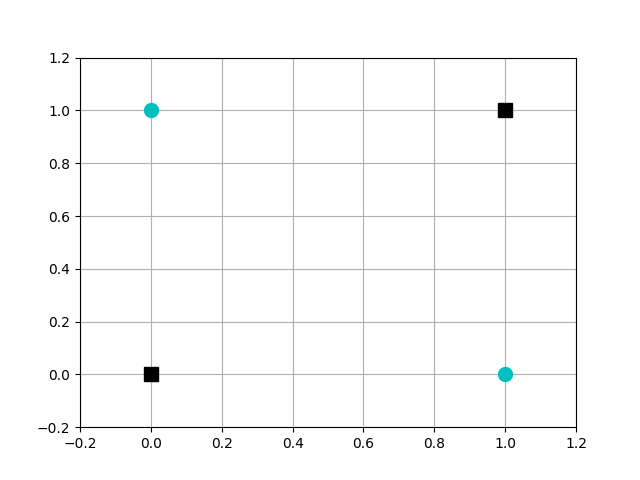
\includegraphics[width=10cm,keepaspectratio,height=10cm]{resources/xor.png}
\caption{Illustration of 4 data-samples representing the XOR problem. Adapted from Figure 13.1 of \cite{pml1Book}.}\label{chap1:xor}
\end{figure}

The estimating of a probability distribution can result in ripping the space into regions when it comes down to classifying inputs to class labels (tasks to their solutions).

The Perceptron algorithm \cite{rosenblatt1958perceptron} was a fundamental precursor of neural networks, and it focuses directly in computing a linear decision boundary for a binary classification task. This translates in finding a good set of weights in the search space of their values, that will define the hyperplane of the boundary. 

We got the following prediction model:

\begin{equation}\label{perc}
    \vect{\hat{c}}= f(\vect{x}) = \mathbb{I}(\vect{w}^T\vect{x} + b)=
    \begin{cases}
        1 \text{ if } \vect{w}^T\vect{x} + b > 0,\\
        0 \text{ otherwise}
    \end{cases}
\end{equation}
the basic idea of the algorithm is to start with random weights, iteratively predict an output for each one of our labeled data $(\vect{x}, \vect{c})$, and update the weights when the model makes a mistake

\begin{equation}
    \vect{w}_{t+1}=\vect{w}_t - \lambda(\vect{\hat{c}}_t - \vect{c}_t)\vect{x}_t
\end{equation}
where $\lambda$ is the \textit{learning rate} or step size.

If the model predicts the correct label at time t, no change is made in the weights from this sample, otherwise weights are moved in a direction so as to make correct predictions more likely.
If $\vect{\hat{c}}_t=1$ was predicted incorrectly, we have $\vect{w}_{t+1}=\vect{w}_t - \lambda \vect{x}_t$. 
If $\vect{\hat{c}}_t=0$ was predicted incorrectly, we have $\vect{w}_{t+1}=\vect{w}_t + \lambda \vect{x}_t$. 

The Perceptron was proven to converge when data is linearly separable.



\subsection{Deep learning}\label{dl}



\subsubsection{Multilayer perceptron}
The \textbf{XOR Problem} from \textit{Perceptrons} \cite{minsky69perceptrons}  was a classic example of a problem that perceptrons, presented in the previous section, cannot solve. A basic case where data is not linearly separable.
We want to represent a function that computes the exclusive OR. So given $\vect{x} \in \{(0,0), (0,1), (1,0), (1,1) \}$, $\vect{c}$ must equal to 1 only if one of the elements of the input is 1 and 0, otherwise. As seen in Figure \ref{chap1:xor}, no linear boundary could be defined, so that samples get correctly classified.






However, with a perceptron, we can model an OR function, and with another one, an AND function since these are linearly separable cases. We could then send our sample $\vect{x}$ to the OR and the AND:
\begin{equation}
    \phi_0(\vect{x}) = \mathbb{I}(\vect{w}^T_{AND}\vect{x} + b_{AND})
\end{equation}
\begin{equation}
    \phi_1(\vect{x}) = \mathbb{I}(\vect{w}^T_{OR}\vect{x} + b_{OR})
\end{equation}
as a result, we would have transformed our input, to another possible intermediate state $\phi(\vect{x}) \in \{(0,0), (0,1), (1,0), (1,1)\}$, where the first coordinate now represents whether the AND was true, and the second coordinate whether the OR was true
\begin{equation}
    \phi(\vect{x}) = \mathbb{I}(\vect{W}\vect{x} + \vect{b})
\end{equation}
now, only the (0, 1) pertains to class 1 (or but not and, thus xor), with which we see that the problem is now linearly separable
\begin{equation}
    f_{XOR}(\vect{x})=\mathbb{I}(\vect{w}^T_{XOR}\phi(\vect{x}) + b_{XOR})
\end{equation}
we have transformed a non-linear separable problem, not solvable by a perceptron, to a linear separable problem, just by joining units of them with specific weight settings (different weights resembling different functions and then different information extracted from the raw inputs in each perceptron unit). See Figure \ref{chap1:xorsolved} for the structure of this process.





%\begin{figure}
%\centering
%\includegraphics[width=10cm,keepaspectratio,height=10cm]{resources/xorsolved.png}
%\caption{XORsolved}\label{chap1:xorsolved}
%\end{figure}


This power of merging multiple simple units to overcome far complex problems is a core idea laying behind neural networks. We have seen in the previous example what is known as a multilayer perceptron. Here, a perceptron resembles what it is known in deep learning as a neuron. The difference is, that perceptron computes a non differentiable function with respect to the inputs received (Eq. \ref{perc}) whereas in neural networks, differentiable \textit{activation functions} are used.

\begin{figure}%
    \centering
    \subfloat[\centering]{{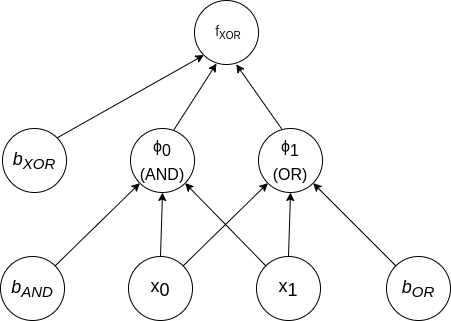
\includegraphics[width=6cm]{resources/xorsolved2.png} }}%
    \qquad
    \subfloat[\centering]{{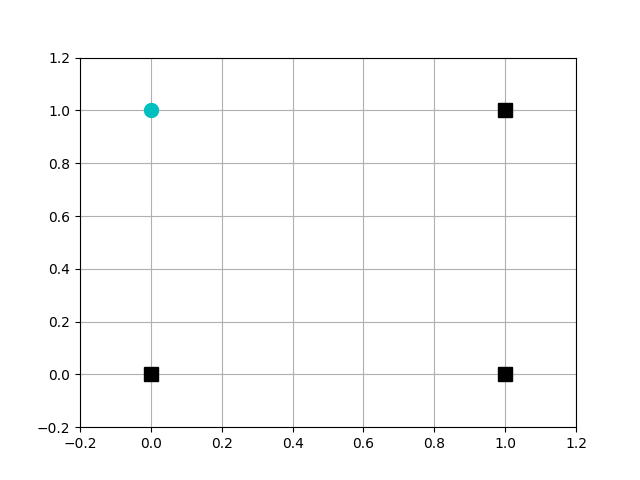
\includegraphics[width=6cm]{resources/xorsolved1.png} }}%
    \caption{(a) Multilayer perceptron solving the XOR problem. (b) Representation of possible output values after the first layer ($\phi$). Adapted from Figure 13.1 of \cite{pml1Book}. }%
    \label{chap1:xorsolved}%
\end{figure}

This is key, because in difference to the example that has been illustrated, the goal and wish of a neural net structure, is to learn the weights of each unit automatically.
Let the model and the optimization process decide which are the weights, for building better functions that transform the input into a problem that is closer to become linearly separable in each \textit{layer}.
%, until the knot is untied at the end of the whole pass through the net.

The model optimization will always depend on the experience that is provided to the system. So it is the data that has been humanly \textit{supervised} what will allow the new unseen data for which we want to predict an outcome to receive a proper answer and the model being a means intermediary facilitating this process.
 

\subsubsection{Neural network}
In a neural network we can have many transformations in chain, $f(x)$ being an arbitrary complex function that can be understood as simpler functions that are nested
\begin{equation}\label{ffnn}
    f(x) = f_L(f_{L-1}(\cdot\cdot\cdot (f_1(\vect{x}))\cdot\cdot \ \cdot))
\end{equation}
where each layer $f_l$ has its own parameters $\vect{W}_l, \vect{b}_l$ and a non-linear differentiable \textit{activation} function $a$ instead of the heaviside function $\mathbb{I}$
\begin{equation}
    \vect{h}_l = f_l(\vect{h}_{l-1}) = a(\vect{W}_l\vect{h}_{l-1} + \vect{b}_l). 
\end{equation}
The first layer of the net receives the raw input $\vect{x}$, while the rest receive the output of the previous \textit{hidden} layer $\vect{h}_{l-1}$.
The last layer is responsible for computing the probabilities for each class, and then usually implements a softmax function with which we can estimate $p(c|\vect{x})$ and output $\vect{c}$ (Eq. \ref{cagmx})
\begin{equation}
    f_L(\vect{h}_{L-1}) = S(\vect{W}_l\vect{h}_{l-1} + \vect{b}_l).
\end{equation}
A neural network can be any model that arranges differentiable activation functions into a directed acyclic graph (DAG), mapping input to output. In (Eq. \ref{ffnn}) we have showcased one of the simplest models, where the DAG is a chain, which we refer to as a Feed Forward Neural Network or FFNN. 
%A FFNN is equivalent to a MLP if we use a specific \textit{loss function}.


The weight parameters of this DAG can be optimized for a \textit{loss function} $\mathcal{L}$ that can be computed for each sample $(\vect{x}, \vect{c})$ comparing the output of the model $\vect{c}_p$ to the true label $\vect{c}$.
We refer to this optimization as the training of the model, which is commonly done using gradient descent and backpropagation \cite{rumelhart1986learning}.

Despite the Perceptron dates from 1958, the XOR Problem from 1969 and backpropagation algorithm from 1986, it was not until recently that neural networks have become a common choice for ML systems.

We can see two first successful usages that improved the state of the art in ML tasks. In 2011 a system was proposed in the automatic speech recognition (ASR) field, which replaced the common choice of Gaussian Mixture Models by a deep approach \cite{dahl2011large} and in 2012 a Convolutional Neural Network (CNN) was showed, which offered a gap in the error rate (from 26\% to 15\% in the top-5 task) for the Imagenet classification task with respect to previous models, that were only improving at a rate of approximately 2\% each year \cite{10.5555/2999134.2999257}.

%showed a CNN that offered a gap in the error rate (from 26\% to 15\% in the top-5 task) for the Imagenet classification task with respect to previous models, that were only improving at a rate of aproximately 2\% each year.

Two reasons that could be attributed to their recent success are that the internet growth has provided large labelled datasets, which allow the training of bigger models without overfit and the increase in computational capacity given by GPUs, specially to perform matrix and tensor operations.

\section{Machine Translation}\label{mt}
The translation of languages is a problem whose automatization has been in research for decades. Many have been the challenges found and the breakthroughs made, as well as the changes of paradigm seen.

The growth in necessity for systems that automatically translated texts (administrative, commercial, entertainment, etc) in all areas of a more multi-lingual and connected world has driven the investments in research that allowed pushing forwards the limits in the field through continued efforts. 

As in any AI task, we want here to see computers showing the appearance of intelligence, the intelligence required to find how a concept encapsulated in words of one language, can be expressed in words of another language. For a person this task often requires profound knowledge of both languages, unravelling meaning and arranging a good representation of it in words from a complete different set, a different language that is influenced by historical, cultural and social factors.

Thus we can see how this mapping can not be most times completely pure, because there is noise in the encapsulating of concepts and in distilling meaning from their representations, even when the process is done by native speakers.

We can distinguish how historical attempts to build translation systems have been based on gathering knowledge of the languages that are to be translated, with the establishment of syntactic and semantic rules built into the system. This involved the work of experts in the languages to build these systems.

However, the predominant and recent trend has been the use of methods that rather rely on data that is available. The model that learns how to perform the task is built up from data. 
%As we've seen, trying to learn how to perform the task with the use of a model that is built up from data. 
This means that we need big sets of well translated sentences on the two languages that we are considering, and from which the model will (learn to) take decisions for future sentences.

\subsubsection{Formal setting}
Machine Translation can be seen as a classification task where the set of possible classes is every sentence that can be produced with the vocabulary of our target language. This is an infinite set of possible classes if we consider sentences of any length, or a very big set if we delimit the max and minimum length of a possible sentence to be produced.

We represent a sentence that is to be translated as a vector of \textbf{n} words $\vect{x} = (x_1,x_2,x_3,...,x_n)$ and its translation as a vector of \textbf{m} words $\vect{y} = (y_1,y_2,y_3,...,y_m)$. These are the \textit{source} and \textit{target} sentences respectively. If we refer to the prediction made by the system we will use $\vect{y}_p$ while if we refer to a given correct translation of sentence $\vect{x}$ we will use $\vect{y}_c$. Note that in difference to the previous Section \ref{sl} we use $y$ instead of $c$ to refer to classes.

As a supervised classification task, our goal is to result in the \textbf{y} that maximizes the probability $p(\vect{y}|\vect{x})$. 
%In this case, result in the best translation possible, the sequence of words $\vect{y}$ that are in most probability a translation of \textbf{x}.
This would be the purest translation of \textbf{x}, the one that matches maximally the concepts that \textbf{x} encloses. We could define though, that a correct translation $\vect{y}_c$ of $\vect{x}$ of language $s$ into language $t$ is one that cannot be distinguished from a translation given by a professional human translator

\begin{equation}\label{nobayesxy}
    \vect{y}_p = \arg \max_{\vect{y} \in Y} p(\vect{y}| \vect{x}).
\end{equation}

As in Section \ref{bayesxc} we can apply Bayes rule to derive  
\begin{equation}\label{bayesxy}
    \vect{y}_p = 
    \arg \max_{\vect{y} \in Y} p(\vect{x} | \vect{y}) p(\vect{y})
    %\arg \max_{y \in Y} p(\vect{y}| \vect{x}) = 
\end{equation}
where $Y$ is the set of possible sentences that can be produced in the language of translation. 

\subsection{Word and Phrase Based Models}\label{wordbased}
We can recall two families of statistical machine translation models that were historically in research and used this decomposition to approximate the probabilities.
These were \textit{word-based} models and \textit{phrase-based} models.
In both, we can distinguish two parts, the \textit{language} model and the \textit{translation} model, which represent the probabilities $p(\vect{y})$ and $p(\vect{x}|\vect{y})$ respectively from (Eq. \ref{bayesxy}).

Word based models \cite{brown1990statistical}, as the intuition their name might give, were models where the translation of a sentence was achieved by computing a best guess for the translation of each word of the sentence.

Phrase-based models \cite{koehn2003statistical}, in contrast, treat a sentence as a sequence of different non-overlapping blocks of words, and then is each one of these blocks which receives its translation to the target language as a unit.

The IBM-1 Machine was an example of a word based model.
For computing an estimation to $p(\vect{x}|\vect{y})$, the translation model, it relied mainly on two aspects. First, a way to learn from well translated sentence pairs what is a best translation for each word individually. This was base based on how each word was most times translated in this data, the real world experience supplied to the system.

Second, a way in which the individually translated words needed to be reordered in the target language of consideration. For this end, it introduced an alignment variable, which defined what was the position in the target sentence, for each word of the source sentence. To learn an estimation for this alignment given a sentence to be translated, it used the EM algorithm \cite{DEMP1977}, again, based too on the information of the language pair present in the human translated parallel corpora which the system had access to.

For an estimation to $p(\vect{y})$, the language model, n-gram models \cite{BRODER19971157} were used.
A language model rather than considering the problem of the language pair, captures information about which words of one language are more likely to appear together in natural expressions of it. In other words, it is a reference of which sentences are more probable than others.

This could help the system to reach decisions when it considers between different translations for the next word, also achieving greater familiarity in the result.
It is a way to incorporate into the system the structure of the language of which we want to produce sentences,  translation sentences in this case. 

The inclusion of a language model allows to make direct use of monolingual corpora of the desired language, which is in most cases more widely available, in greater amounts and more easily gathered.

A way one could approximate $p(\vect{y})$ would be to think of which is the probability of the next word $y_n$ in a sentence given the previous words, and then give the probability for the whole sentence using the chain rule.
%\begin{equation}
%    p(\vect{y}) =  p(y_n | y_{n-1}, y_{n-2}, ..., y_0)p(y_{n-1} | y_{n-2}, ..., y_0)\times ...\times p(y_1 | y_0)p(y_0) 
%\end{equation}
\begin{equation}
    p(\vect{y}) = p(y_0) \prod_{n=1}^{N} p(y_n | y_1^{n-1})
\end{equation}
Given that the number of different possible preceding words grows exponentially, a n-gram model makes the assumption that the word at position i will depend on the context of only n preceding words, thus taking into account a limited history and achieving computational feasibility.

As for phrase based models, it was log linear models which were a notorious example.
Their language model was also estimated using n-grams, whereas the translation model was formed by two parts, a \textit{lexicon translation} model and a \textit{reordering} model. 
Although we will not dive into an explanation of these constituents, they were the state of the art for the machine translation task before deep neural networks took main presence.


\section{Neural Machine Translation}

As we have seen in Section \ref{dl}, the use of neural networks for classification tasks started to show results that created performance gaps in comparison to non-deep systems. FFNNs worked for structured data and CNNs worked best for images. As these outcomes appeared each time more present, deep models were also brought to the translation framework.

In this scenario where data was unstructured, in form of sequences of variable length, RNN architectures were the main actors to take part.
First, deep learning approaches were used to replace only certain parts of the systems, while the first model using a net for the whole translation pipeline was a RNN with an attention mechanism \cite{https://doi.org/10.48550/arxiv.1409.0473}.


\subsection{RNN and Translation}\label{nmtrnn}

Different tasks can be tackled in the scenario of working with sequences, and then different structures for RNNs can be seen. We could want the output to be a vector of labels into which classify an input sentence (for example whether a statement is negative, positive or neutral) or the inverse problem, given an input in form of a vector, we could expect a sequential output (e.g. image captioning generation). However, we will focus in the problem called sentence translation (language translation in this case) which maps sequence to sequence. See Figure \ref{chap1:seq2seq} for a representation of a sequence-to-sequence RNN.

\begin{figure}
\centering
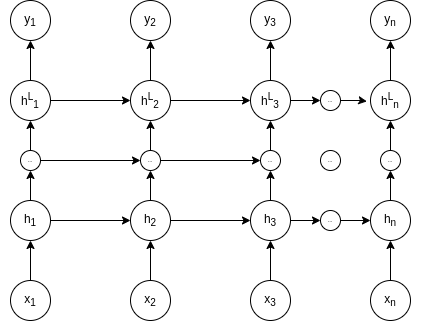
\includegraphics[width=10cm,keepaspectratio,height=10cm]{resources/seq2seq.png}
\caption{Sequence to sequence recurrent neural network with $n$ hidden states and $L$ hidden layers. Adapted from Figure 15.5 of \cite{pml1Book}.}\label{chap1:seq2seq}
\end{figure}

A Recurrent Neural Network is a neural network which incorporates an internal \textit{hidden} state $\vect{h} = (h_1, h_2, ..., h_T)$ where $T$ is the length of the output. The output produced in the model will then depend on this hidden state in addition to the input introduced in the system.
The key to working with sequences is that the internal state of the model will be updated word per word along the processing of $\vect{x}$. 

This means, it will capture information about the preceding words (or future words of the sequence too in a Bidirectional RNN \cite{650093}) when working at word at position $n$
\begin{equation}
    p(\vect{y}|\vect{x}) = \sum_\vect{h} p(\vect{y},\vect{h}|\vect{x}).
\end{equation}

These models and the later transformer  architecture, model $p(\vect{y}|\vect{x})$ directly (Eq. \ref{nobayesxy}), in contrast to the non-neural approaches described in Section \ref{mt}. Even if we denote \textbf{n} as the length of the input sequence, a RNN expects inputs of variable \textbf{n}, while in a FFNN for example, once the model is defined, the input length remains constant.

Each state $h_t$ could be built as a LSTM unit \cite{hochreiter1997long} or a GRU unit \cite{cho-etal-2014-learning}, that determines which information should be kept from the previous state $h_{t-1}$ and from the upcoming word $x_t$, to be passed to the next state. If we combine two RNN  one building $\vect{h}$ from the start of the sentence to the end and the other in inverse order, we would be describing a Bidirectional RNN
\begin{equation}\label{hfor}
    h_t^\rightarrow = \varphi (\vect{W_x}^\rightarrow x_t^\rightarrow + \vect{W_h}^\rightarrow h_{t-1}^\rightarrow + \vect{b}^\rightarrow )
\end{equation}
\begin{equation}\label{hback}
    h_t^\leftarrow = \varphi (\vect{W_x}^\leftarrow x_t^\leftarrow + \vect{W_h}^\leftarrow h_{t+1}^\leftarrow + \vect{b}^\leftarrow )
\end{equation}

\begin{equation}
h_t = [h_t^\rightarrow, h_t^\leftarrow]
\end{equation}

where $\varphi$ would be a differentiable nonlinear function. 
The state $h_t$ represents then information the past (words prior to $x_n$) as well as information of the future.

When we reach the final word of the sentence $(t=T)$, $\vect{h}$ has been built upon preceding states $h_{t-1}^{h_1}$ and all words have been read. Thus we can see $\vect{h}$ as a representation of the information the sentence contained.

This addresses one basic problem in the translation pipeline. How to represent sentences that are verbal human compositions, in a numerical computer-readable arrangement.

Since we are in a deep learning framework, which information is extracted from the words will depend on the values of weight matrices as we see in (Eq. \ref{hfor}), (Eq. \ref{hback}), and the task of discovering which is a proper set of weights is then let to the network to be optimized through backpropagation.

Once this representation of the input data is produced by the model (being the output of this network the last hidden state itself), we could use another RNN, that learns the inverse problem. Receiving $\vect{h}$ as input, produce word per word a sentence, but in the desired language of translation. The internal state $\vect{s}$ of this \textit{decoding} RNN would be updated with the preceding state together with the word the system just previously produced until the end of sentence is brought out.
\begin{equation}\label{sdec}
    s_t = \varphi (y_{t-1},s_{t-1})
\end{equation}

This scheme where input information is encoded in a subspace and then decoded into the solution of the problem, can be seen in general under the name encoder-decoder, where each module is not necessarily implemented by a RNN nor a NN.

As mentioned in the beginning of this section, it was the model used in \cite{https://doi.org/10.48550/arxiv.1409.0473}, with a BiRNN as encoder and a RNN as the decoder.

This was the first standalone neural model for machine translation, i.e. the first translation system where the whole model was a single neural network (3 RNN working together) and the whole trained together at a time.

It included though an element of main relevance, an \textit{attention mechanism} that modified the update step of the internal state in the decoder (Eq. \ref{sdec}) RNN to depended on an extra \textit{context} vector $\vect{c_t}$.
\begin{equation}\label{decoc}
    s_t = \varphi (y_{t-1}, s_{t-1}, \vect{c_t})
\end{equation}

\subsubsection{Attention mechanism}

Attention is a technique that (in a RNN) allows a state $h_t$ to receive information directly from any other state $h_y$ in the network. If we see $h_t$ as the representative of meaning when looking a sentence at position $t$, with attention we build a structure in the network that allows it to learn which states are more dependent on each other, and thus should be most taken into account when building each other state. 

We could imagine a scenario where the meaning of a word in a sentence is understood in relation to other distant words. Attention would allow a connection between these, that otherwise might have been lost along all updates of \textbf{h}. Having this extra information allows better representations, leading to better results. And are the better results during training of the net which guide the building (or discovery) of these dependencies.

Following \cite{pml1Book}, attention can be described as a dictionary lookup where for a query \textbf{q} and a set of keys $\vect{k_i} \in \vect{K}$, we compute a combination of the values $\vect{v_i} \in \vect{V}$.

\begin{equation}\label{attn1}
    Attn(\vect{q}, (\vect{K}, \vect{V})) = \sum_i \alpha_i(\vect{q}, \vect{K})\vect{v_i}
\end{equation}
the strength of the connection between the query \textbf{q}  and the key $\vect{k_i}$ is modelled by the \textit{attention weight} $0\leq \alpha_i(\vect{q},\vect{K})\leq1$
\begin{equation}\label{attn2}
    \alpha_i(q,K) = S_i(a(\vect{q},\vect{k_1}), ...,a(q, \vect{k_n})) = \frac{\text{exp}(a(\vect{q},\vect{k_i})}{
    \sum_j^n \text{exp}(a(\vect{q},\vect{k_j}))}
\end{equation}
where $S$ is the softmax function and defining $a$ in the following way gives name to what is called \textit{scaled dot product attention}:
\begin{equation}\label{sdpa}
    a(\vect{q},\vect{k}) = \frac{\vect{q^T}\vect{k}}{\sqrt{d}} 
\end{equation}
where $d$ is the length of both the query and key.

In the context of a RNN with hidden states representing the meaning of words, attention could compute the dependency of hidden state $h_t$ to each other state $h_i$
\begin{equation}\label{attnRnn}
    Attn(h_t, (\vect{h}, \vect{h})) = \sum_{i=1}^T \alpha_i(h_t, \vect{h})h_i.
\end{equation}

Thus attention when focusing on a sentence position will be a combination of the hidden states, where the states will have a bigger or smaller weight depending on how their dependency to the word at that position is relevant for producing better results. We allow the network setting low weights for some states (ignoring parts of the sentence for this word) or emphasizing the meaning other parts (high attention weight values).

It has been observed that systems that did not use attention provided worse results, specially when working with long sentences where these distant dependencies are hard to handle by a native RNN in its hidden state.

In the neural network system for translation that we have previously referenced \cite{https://doi.org/10.48550/arxiv.1409.0473}, each state $\vect{s_i}$ of the decoder attended not its own hidden states but the hidden states of the encoder. This allowed to dynamically focus on parts of the source sentence upon each production of a word for the target sentence.

If we recall (Eq. \ref{decoc}) we can now define the context vector $\vect{c_t}$
\begin{equation}
    \vect{c_t} = \sum_{i=1}^T\alpha_i(s_{t-1},\vect{h})h_i.
\end{equation}
The attention weights, can be seen acting as an alignment of target words to source words.

\subsection{The Transformer Model}
If the first neural standalone model was released in 2016, it was not long before the Transformer model was published in 2017.
If models using attention were showing state of the art results in the area, the transformer based its architecture fully on it.

Also following an encoder decoder scheme, attention is used in both parts, learning the representation of data during encoding as well as producing each resulting word in the decoder.
Given the wide employment of the model, there are many good references that explain it \cite{https://doi.org/10.48550/arxiv.1706.03762}, \cite{pml1Book}, \cite{zhang2021dive}, \cite{koehn2020neural}, in addition to its many variations.

Since it is the model at the core of the systems developed in this work, we will describe the architecture and its fundamental features, so the reader can have a realistic grasp on the tasks carried out along the project.

\subsubsection{Self Attention Architecture}
From a zoomed out view, the Transformer is built of a stack of encoding units on top of each other, which pass their information to another stack of decoding units at the top of which output words are produced. We can see a representation of the structure in Figure \ref{chap1:transformer}.
The model can be understood understanding these two kinds of units (see Figures \ref{chap1:encode} (a) and \ref{chap1:encode} (b) for the encoding and decoding units respectively).

\begin{figure}
\centering
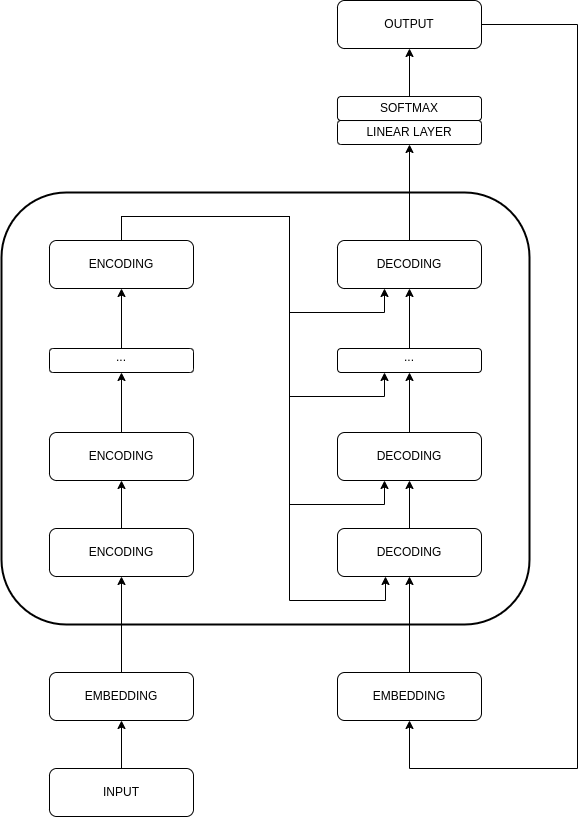
\includegraphics[width=12cm,keepaspectratio,height=10cm]{resources/transformer.png}
\caption{A structural representation of the Transformer model with a certain number of encoding and decoding units.}\label{chap1:transformer}
\end{figure}

When a sentence is supplied to the system, we do not have now a hidden state, so instead of processing it word per word as in a RNN, attention is performed to each word with respect to each other word of the sentence hence called \textit{self} attention. This becomes the new representation of the word, that has gathered valuable context from the other words. 

The new representations are passed to the next encoding unit (after extra process as seen in Figure \ref{chap1:encode} (b) ), that will perform the same operations.
This change in architecture allows high parallelization that results in training and inference speed improvements.


\begin{figure}%
    \centering
    \subfloat[\centering]{{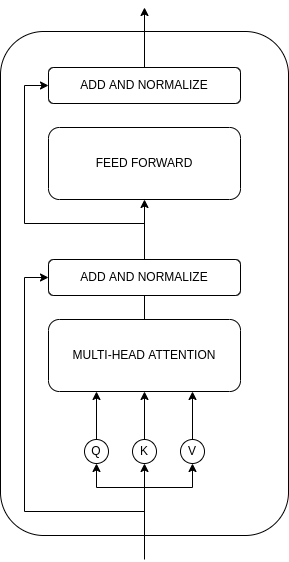
\includegraphics[width=4cm,height=7cm]{resources/encode.png} }}%
    \qquad
    \subfloat[\centering]{{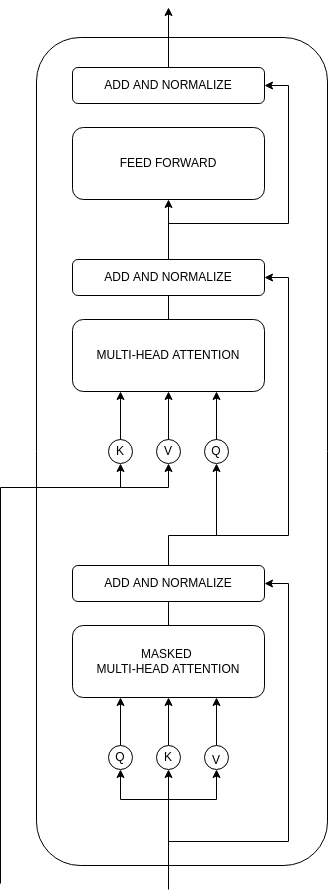
\includegraphics[width=4cm,height=10cm]{resources/decode.png} }}%
    \caption{(a) Representation of a encoding unit from Transformer. (b) Representation of a decoding unit from Transformer where $K$ and $V$ values are obtained from the top-most encoding unit. }%
    \label{chap1:encode}%
\end{figure}

If input word is $\vect{x_i}$ and output word $\vect{o_i}$ after one attention layer, 
\begin{equation}
    \vect{o_i} = Attn(\vect{x_i}, (\vect{x_1}, ...,\vect{x_n}), (\vect{x_1}, ...,\vect{x_n}))
\end{equation}

in practice attention is carried out through matrix operations, all queries arranged in matrix $\vect{Q}$.
We keep using scaled dot product attention (Eq. \ref{sdpa})
\begin{equation}
    Attn(\vect{Q}, \vect{K}, \vect{V}) = S(\frac{\vect{QK^T}}{\sqrt{d}})\vect{V}.
\end{equation}

\subsubsection{Multi Head Self Attention}
In addition to this new base idea for learning the representations for the words, we don't only have one set of attention weights per word but as many \textit{heads} as we define. This means that multiple dependencies or similarities can be captured for a word with respect to all other words in the sentence for each head, with a different set of weights specialized for each one of these dependencies.

For example, if we consider the word 'it' in a sentence, one set of weights could focus on which subject this pronoun refers to, while other attention head could focus on adjectives that are describing it
\begin{equation}
    \vect{head_i}=Attn(\vect{Q}\vect{W^q_i}, \vect{K}\vect{W^k_i}, \vect{V}\vect{W^v_i})
\end{equation}
where queries, keys and values have been linearly projected to other subspaces by the trainable matrices $\vect{W_i^q}, \vect{W_i^k}, \vect{W_i^v}$.

Heads are concatenated, and to restore the original dimension, multiplied by $\vect{W^o}$
\begin{equation}
    \text{MultiHead}(\vect{Q},\vect{K},\vect{V}) = \text{Concat}(\vect{head_1},...\vect{head_h})\vect{W^o}
\end{equation}

Multihead attention is applied in the encoder stack as we have described, while in a decoding unit, it is applied in two different ways.

For an output word being produced, the aim is to receive information from the source sentence words as well as the already translated output words. This is why, words of the target sentence go through a first layer of self \textit{masked} multi head attention.

This restricts the mechanism of attending words that have not been yet translated. Even if during training time all correct translations are known, it is not the case once the system is in production. That's why the model has to learn to translate without relying on this information.

Successively after this layer, there is a layer of multi head attention that attends source sentence information. Queries are the current representation for output words $\vect{y_i}$ and keys and values are each of the positions of the output of the encoding stack (see Figure \ref{chap1:transformer}).

So in a decoder unit, better representations are learnt from previous translated words, and then the information of the encoding part is gathered too. These operations are repeated in chain for each unit until the top of the decoding stack is reached.

\subsubsection{Layer Normalization and Residual Connections}
As we see in Figures \ref{chap1:encode} (a), \ref{chap1:encode} (b) in addition to attention layers, FFNNs (Eq. \ref{ffnn}) are used to build the units in this case with ReLU activation functions \cite{https://doi.org/10.48550/arxiv.1803.08375}.
After both, FFNN or attention, \textit{layer normalization} \cite{ARTS:LayNor} and \textit{residual connections} \cite{7780459} are performed.

These are common techniques in NN that help the optimization process of the net. 
Layer normalization aims to prevent the problem of vanishing and exploding gradients (see \cite{pml1Book} Section 13.4.2), while residual connections allow the backward flow of gradients during backpropagation even when gradient vanishing occured in parts of the net. They allow training deeper models with much bigger number of layers.

Residual connections allow the input of a layer to \textit{skip} all the transformations F that the layer perform to x, thus add x at the output of the layer.
\begin{equation}
    F'(x) = F(x) + x
\end{equation}
$F'(x)$ being the output of the residual block.

Layer normalization computes the mean and variance across outputs of hidden units of a layer before the activation function
\begin{equation}
    a_i^l = w_i^{l^T}h^l \ \ \ ; \ \ \ h_i^{l+1} = f(a_i^l + b_i^l)
\end{equation}
\begin{equation}
    \mu^l=\frac{1}{H}\sum_{i=1}^{H}a_i^l \ \ \ ; \ \ \ \sigma^l=\sqrt{\frac{1}{H}\sum_{i=1}^H(a_i^l-\mu^l)^2} 
\end{equation}
where $w_i^l$ are the weights of hidden unit $i$ and $h_l$ the inputs received from the previous hidden layer $l$.
Then the variance is divided element-wise and the average is subtracted
\begin{equation}
    \text{LayerNorm}(a^l) = \gamma \frac{a^l-\mu^l}{\sigma^l} + \beta.
\end{equation}
The next layer becomes then
\begin{equation}
    h^{l+1}=f(\text{LayerNorm}(a^l) + b^l)
\end{equation}
$\gamma$ and $\beta$ being trainable weights that allow the net to undo these changes partially or completely favouring the optimization.

\subsubsection{Input representation and positional encoding}\label{inputrep}

If we recall RNNs, words were processed sequentially, and hidden states updated accordingly in a sequential fashion, thus capturing information about the position occupied by each word in the sentence. 

This is not the case in the Transformer since attention is invariant to the ordering of the words. To provide the model with this information, a \textbf{positional encoding} is combined with the \textbf{word embedding}.

When a sentence goes into the model, prior to transforming it through all attention layers, we need to change from a natural language representation to a numerical one, and so each word is first transformed to a one-hot vector, that represents its corresponding index in the vocabulary. So a sentence would be represented in a matrix of size ($n \times vocabulary\_size$), where $n$ is the number of words.

After this, it is multiplied by a learnt embedding matrice $\vect{E_e}$, of size ($vocabulary\_size \times d$), where $d$ is a parameter of the model. Words are projected to this dimension, ending with a representation of a sentence in dimension ($n \times d$). This is the word embedding $\vect{WE}$
\begin{equation}
    \vect{WE} = \vect{x} \vect{E_e}
\end{equation}
where x is the one-hot representation of the input sentence.
Now, to account for position information, we build a matrix also of dimension ($n \times d$) where each row represents the position of a word in a d-dimensional vector. This matrix could also be learnt, but the Transformer uses a fix encoding instead, that is given by two sinusoidal functions
\begin{equation}
    \vect{PE}_{(pos,2i)} = sin(pos/10000^{2i/d})
\end{equation}
\begin{equation}
    \vect{PE}_{(pos,2i+1)} = cos(pos/10000^{2i/d})
\end{equation}
where $pos$ is the position of the word in the sentence, and the corresponding row of the $\vect{PE}$ matrix, and $i$ each index of this row
\begin{equation}
    Embedding(\vect{x}) = \vect{WE} + \vect{PE}.
\end{equation}

This choice for the positional encoding provided no performance decrement compared to a learnt embedding, while allowed the model to extrapolate to sentence lengths that were unseen during training.

Exactly the same process is applied to source words on the encoding as to words that enter the decoder stack ($y_0^{t-1}$ produced by the decoder in previous instants).

The Transformer model also uses a technique called Weight Tying \cite{press-wolf-2017-using}
where a single matrix $\vect{E}$ is used for the encoding as for the decoding, and also for the output embedding matrix$(\vect{E_o}=\vect{E^T})$, that transforms the output of the last hidden layer in the encoder into probabilities for the next word when given to the softmax layer after a learnt linear transformation.

Transformer architectures have shown success with state of the art results in MT as well as in a wide range of NLP tasks. We can name language modelling, document summarization, sentiment analysis, text generation, text paraphrasing, reading comprehension or question answering.
The systems GPT-3 \cite{https://doi.org/10.48550/arxiv.2005.14165}, BERT \cite{https://doi.org/10.48550/arxiv.1810.04805}, or T5 \cite{https://doi.org/10.48550/arxiv.1910.10683} are developed on Transformer architectures. Whenever we think of a task that involves working with language or see a translator offering good results in production, there is probably a Transformer operating in behind.

Recent results of the 2022 IWSLT competition \cite{anastasopoulos-etal-2022-findings} show the wide and present use of the Transformer model for machine translation tasks.

\section{Evaluation}

Evaluation of MT systems is an active research area. Quantifying the quality of the translations that our systems produce is essential towards developing better models that outperform precedent systems, since we need ways to know that the results are indeed better. Manual evaluation of the translations would let us know with high reliability what is the performance of our systems, since the judgment of target translations would be done by humans who have knowledge of what are truly correct translations. However, the need of evaluating the performance of MT systems is very frequent, hence there is need to find automatic measures which correlate with human evaluation. 

A dominant metric for MT tasks is BLEU \cite{papineni-etal-2002-bleu} which stands for Bilingual Evaluation Understudy. It is a measure of \textit{precision} between target translations (the ones produced by our systems) and \textit{reference} translations which we have available as part of our parallel datasets. 
Simple precision is computed as the number of words in the target translation that are also present in the reference translation, divided by the total number of words in the reference translation. 
Measuring only this precision does not take into account the context information of other words in the sentence, does not penalize the production of short target sentences, and can be unreliable, since producing outputs which contain very frequent words of the target language, but that are not related to the meaning of the source sentence, could lead to high precision scores.

Instead, BLEU computes a precision $p_n$ at different orders of n-grams. This precision is \textit{clipped}, so that in contrast to normal precision, n-grams of the produced translation are only counted once for each time they appear in this translation, even if in the reference translation there are more instances of these n-grams 
\begin{equation}
    AveragePrecision(N) = \frac{1}{N} \sum_{n=1}^Nlogp_n.
\end{equation}

In addition to this, BLEU computes a brevity penalty, which is applied when the target translation $\vect{y}_p$ is shorter than the reference translation $\vect{y}_c$

\begin{equation}
BrevityPenalty=
\begin{cases}
1 & |\vect{y}_p| > |\vect{y}_c| \\
exp(1-\frac{|\vect{y}_c|}{|\vect{y}_p|}) & |\vect{y}_p| \leq |\vect{y}_c| \\ 
\end{cases}
\end{equation}.

BLEU is then computed using n-grams of up to 4 tokens

\begin{equation}
    BLEU(4) = BrevityPenalty \cdot AveragePrecision(4).
\end{equation}

This gives a final value between 0 and 1 which is multiplied by 100 for easier readability. We will use this metric to evaluate the performance of our different models implemented in this work. According to the interpretability research conducted at \cite{specia-etal-2009-improving}, we can contextualize BLEU scores where results above 40 are regarded as a system which produces target translations of good quality, which need little human post-editing. Results above a 30 require post-editing in order to be correct translations, but still the amount of post-editing work would be less than the effort of translating manually the sources from scratch. 
%Refer to the usefulness of BLEU!!!!!!!!

%We have to undo the preprocessing steps for evaluation%Sacrebleu

%Bleu \cite{papineni-etal-2002-bleu}
%sacrebleu \cite{DBLP:journals/corr/abs-1804-08771}

\section{Framework of this work}\label{framework}
This work has been developed during and thanks to the author's research internship at the Valencian Research Institute for Artificial Intelligence’s Machine Learning and Language Processing (VRAIN-MLLP) research group at Universitat Politècnica de València (UPV). In this context, the systems developed aim to contribute to the work carried out for a techonlogy-transfer contract between the CERN and the MLLP group. This includes automatic captioning and translation systems for CERN's multimedia sources, as well as low-latency translation systems for webcasts and conference meetings of CERN's internal and external communication systems. We present the process and results of developing domain-adapted offline and streaming MT systems for English to French translation. In this case MT systems are adapted to the high energy physics domain, which is highly present on the CERN contents.


\section{Document structure}

This document is organized in 7 chapters. This first chapter introduces the context of this work in artificial inteligence up to the more specific fields of machine learning and neural machine translation. It describes the theoretical concepts and models that we will employ during the development of this work such as the state of the art Transformer architecture, as well as precedent models. In addition to this, it explains how we will evaluate our systems, which are our goals and motivations, as well as the framework in which the tasks to be carried out are developed. 

In Chapter \ref{dos}, we describe the data preprocessing techniques that we will use in our systems, as well as the general domain corpus and datasets that will be employed for different tasks in our systems, such as training and evaluation. In Chapter \ref{tres}, we move on to explain the process of compiling a domain specific dataset that we will use to perform domain-adaptation and evaluation of our systems.

Chapter \ref{systems} describes the computer toolkit that we will use to implement and make use of our models, as well as the detailed explanation of the different experiments and results that we developed for offline machine translation systems, comparing them to an already working model. In Chapter \ref{domad} we describe two different techniques of adapting general-domain purpose systems to in-domain scenarios, and describe the experiments and results carried out to adapt in this way our previous models.

In Chapter \ref{strnmt}, we move to the scenario of streaming machine translation, detailing formally this new framework, explaining the theoretical model that we will use and the different evaluation metrics of latency for this kind of systems. Finally in this chapter, we present the implementation of one model of this kind together with the results of such model. The work concludes with Chapter \ref{conclusion} summarizing the tasks carried out along the different chapters as well as covering the conclusions reached in these tasks.


%\section{Notes bibliografiques} %%%%% Opcional

%????? ????????????? ????????????? ????????????? ????????????? ?????????????

%%%%%%%%%%%%%%%%%%%%%%%%%%%%%%%%%%%%%%%%%%%%%%%%%%%%%%%%%%%%%%%%%%%%%%%%%%%%%%%
%                         CAPITOLS (tants com calga)                          %
%%%%%%%%%%%%%%%%%%%%%%%%%%%%%%%%%%%%%%%%%%%%%%%%%%%%%%%%%%%%%%%%%%%%%%%%%%%%%%%

\chapter{Data}\label{dos}
In this chapter we will describe the data that we will be using in our systems, as well as the different processing techniques that this data will undergo prior to any use of it by our models. 

\section{Datasets}
As we have described in Chapter \ref{intro}, all learning and thus all performance that our systems will achieve will be based on the real world experience that we make them available with.

In our MT scenario where data consists of sentences paired with their translations, the model will assume that the translation that we give is correct. Thus if we offer the system with incorrect translations, this will be reflected in the system performance, since predictions will be based on these false truths. With this we can understand how the quality of the data is important in building our systems.

The quantity of data is another main factor with what respect to system results. The Transformer is a big architecture that allows us to train with datasets consisting of millions of sentence pairs. Systems offering state of the art performance are usually trained using very big datasets, that allow us to train without overfit, these big models that have billions of parameters. For example, GPT-3 \cite{https://doi.org/10.48550/arxiv.2005.14165} is trained with a dataset consisting of approximately 499 billion of words.

This opens a trade-off, since there is a need for large amounts of data, but manual production is highly resource consuming for many tasks. It is so specially in MT where we need paired sentence translations, and we could potentially want to translate between many different language pairs. In this labour, there are many collaborative works that have achieved the compilation of big public parallel datasets. We can refer to OPUS \cite{aulamo-tiedemann-2019-opus} as a work that tries to gather in a single open site, big part of the available datasets for machine translation.

In a supervised machine learning framework and specially in a classication task, we can distinguish between three different types of sets. These are training, development and test sets. Comparably in size, a training set tends to be much bigger than the development and test sets, and this is the case in the NMT scenario, as we will see, by orders of magnitude. The latter two, are sets devoted to evaluating our model. The main difference between a development and a test set, is that the development set is used to perform parameter exploration of our models, and choose different configurations depending on the results on this set. Also, it can be used to measure the performance of the system while the training is ongoing, to see for example if the system is performing too well on the training data, while decreasing the quality in the development set which is not used for the optimization process of the model. In contrast, a test set is designed to be a final measure of the performance of our system, mimicking the performance that the system will have on completely unseen data once it is in production.

The sets that we present in this chapter are those of general-domain data. Data that is not specific of any context and rather gathers sentences of many different kinds, as source for general-purpose translation systems. 

We will see in Chapter \ref{domad} how having prior knowledge about the phrases that our model will translate, can be used for building a model that performs better for this data, with a process that encloses a set of different techniques known as \textit{domain adaptation}. For these techniques, we often use sources of \textit{in-domain} data, which contain sentences with similar context and similar vocabularies as those the model will have to translate, the specific context to which we refer as the \textit{target} domain.

%General/In domain data
%Development & test

%Left ideas
%Monolingual are easier to gather
%Crawling needs filtering and processing and automate tools to clean corpus
%There are other ways rather than crawling
%Parliments, books
%Before crawling  
\subsection{General domain training dataset}\label{dataset}
Our training dataset has been compiled with the purpose of training a general domain translation model i.e. a model built for translating sentences of the English language without making assumptions of their contents. In this way, we have gathered open sources that contain sentences of very different contexts, with no fixation on any in particular. We can see a summary of the dataset in Table \ref{chap2:trainset}. 

%\begin{figure}
%\centering
%\includegraphics[width=10cm,keepaspectratio,height=10cm]{resources/trainset.png}
%\caption{trainset}\label{chap2:trainset}
%\end{figure}

\begin{table}
\caption{Statistics on parallel datasets. M = $1\cdot10^6.$}
\centering
\begin{tabular}{l|c|c|c}
 & Sentence pairs & English words & French words\\
\hline
    CommonCrawl & 0.1M & 4.1M & 4.7M \\
    CCAligned & 15.6M & 156.7M & 171.1M \\
    ParaCrawl & 216.6M & 3700M & 4100M \\
    WikiMatrix & 2.7M & 57.8M & 63.1M \\
    WikiMedia & 1.0M & 24.1M & 25.8M \\
    Giga Fr-En & 22.5M & 575.8M & 63.1M \\
    UNPC & 30.3M & 658.4M & 816.4M \\
    EUBookshop & 10.8M & 224.6M & 244.5M \\
    Europarl & 1.2M & 28.6M & 29.9M \\
    Europarl-ST & 96500 & 2.3M & 2.6M \\
    DGT-TM & 4.9M & 86.3M & 95.4M \\
    News Commentary & 3.2M & 70.7M & 76.6M \\
\hline
    Total & 309M & 5600M & 6300M \\
\end{tabular}
\label{chap2:trainset}
\end{table}



We count up to 309 million sentence pairs in our dataset, which makes a total of $5.6 \cdot 10^9$ words for the English language and $6.3 \cdot 10^9$ words for the French language.

A portion of the datasets that we use are built crawling parallel text resources from the web. In this task, automatic tools to process and cleaning the data are determining to produce sets of good quality. Of this kind we have:
\begin{itemize}
    \item CommonCrawl\footnote{https://commoncrawl.org/the-data/}, CCAligned \cite{el-kishky-etal-2020-ccaligned} and ParaCrawl \cite{banon-etal-2020-paracrawl} from different sources of the web.
    \item WikiMatrix \cite{DBLP:journals/corr/abs-1907-05791} and WikiMedia \cite{tiedemann-2012-parallel} sourced from Wikipedia.
    \item Giga Fr-En \cite{TIEDEMANN12.463} crawled from Canadian and European Union sources for the WMT2010 Competition \footnote{https://www.statmt.org/wmt10/translation-task.html}.
\end{itemize}

The rest of the parallel sets that form our training data can be classified in a group of sources that have not been gathered from the web:
\begin{itemize}
    \item The United Nations Parallel Corpus (UNPC \cite{ziemski-etal-2016-united}) from manual translations of United Nations documents ranging from 1999 to 2014.
    \item EUBookshop \cite{skadins-etal-2014-billions} from publications of European institutions.
    \item Europarl \cite{koehn-2005-europarl} and Europarl-ST \cite{DBLP:journals/corr/abs-1911-03167} from the European Parliament.
    \item DGT-TM \cite{DBLP:journals/corr/SteinbergerEKPS13} published by the same DGT (Directorate-General for Translation), a department in the European Commission and one of the biggest translation services in the world.
    \item News Commentary \cite{TIEDEMANN12.463} a collection of News Commentaries provided by WMT and sourced from CASMACAT\footnote{http://www.casmacat.eu/corpus/news-commentary.html}.
\end{itemize}

%Idees en memoria Javi 
%Vocabulary size is important
%lowercase truecase (predicts capitalization for each word)
\subsection{Development and Test Datasets from WMT}
The WMT Conference on Machine Translation (originally Workshop on Machine Translation) is a main event in the field of Machine Translation Research.
The conference is held annually, where universities, research laboratories and technology companies participate pushing performance boundaries of the systems for a set of proposed machine translation tasks.
We have decided to evaluate the performance of our system with the tests sets of the WMT13\footnote{https://www.statmt.org/wmt13/translation-task.html} and WMT14\footnote{https://www.statmt.org/wmt14/translation-task.html} competitions.
These are general domain data of high quality.

Since development and test sets in machine translation are relatively much smaller than training sets (of orders of thousands of sentences) they can be reviewed in detail for adequate translations, assuring to be works useful to contrast the quality of our translations.
We use WMT13 and WMT14 respectively as the principal development and test sets for measuring the performance of our systems for general domain. 

%We will see in Chapter \ref{domad} the use of a different development and test set to evaluate the performance on a specific domain.

\section{Preprocessing}
%If we emphasized that learning is from data, we emphasize now that how is this data also plays inmense role
Data preprocessing is a common step in NMT systems prior to feeding our models with this data either for training or for inferring the translations. It works improving the quality of the results as well as the computational efficiency and feasibility of the models. We will now describe the different techniques that we used when developing our systems.

\subsection{Tokenize and Truecasing}
To understand these steps we need to understand that our systems work with a vocabulary of fixed and limited size i.e. a limited number of words that will be recognized from the English language and a limited number of words that will be possibly produced in French (we will see in Section \ref{subw} techniques to pragmatically overcome this limitations even if keeping the vocabulary fixed and limited). 

If we refer to Section \ref{inputrep} we see that the size of the one-hot vectors representing each word of an input sentence depends directly on the vocabulary size of the source language, while the size of the final softmax layer of the model(see Figure \ref{chap1:transformer}) that accounts for probabilities for each next word, depends on the size of the output vocabulary. In this way, reducing vocabulary sizes translates in reducing memory consumptions and increasing computational efficiency.

If we considered each sequence of symbols that is separated by blank spaces to be a word of our vocabulary, we would encounter that we could have many different word instances that represent the same word. Consider the example \textit{Okey!} \textit{Okey...} \textit{Okey,} \textit{Okey?}.
These four would be considered individual words of our vocabulary, which would grow extensively big. 
We leave then the task of deciding what constitutes a word to a \textit{tokenizer}, that in this case would separate the word \textit{Okey} from punctuation, and treat each part as an individual \textit{token} of the vocabulary. %See figure (\ref{chap2:tok}) for an example of \textit{tokenization} performed in our systems.

%\begin{figure}
%\centering
%\includegraphics[width=10cm,keepaspectratio,height=10cm]{resources/tokenize.png}
%\caption{tok}\label{chap2:tok}
%\end{figure}


An additional step that reduces the size of our vocabularies consists in dealing with upper and lowercase letters. Instead of keeping diverse versions for a word (consider for example \textit{ATTENTION}, \textit{Attention}, \textit{attention}), we train a \textit{truecasing} model that predicts which case should be kept based on the frequency of each case of each word in our data. 
A simpler approach to this issue would be to lowercase all words, but more linguistical information would be lost.

In our work we use the Moses tokenizer and truecasing \cite{koehn-etal-2007-moses}. We can see an example of their usage in Table \ref{table:truec}.

%estic aci
%Mrs Plooij-van Gorsel, I can tell you that this matter is on the agenda for the Quaestors' meeting on Wednesday.

%Mrs Plooij @-@ van Gorsel , I can tell you that this matter is on the agenda for the Quaestors ' meeting on Wednesday .


\begin{table}
    \caption{Training sentence before and after applying Moses' truecasing and tokenizer.}
\centering
\begin{tabular}{|c|l|c}
\hline
    Original & Mrs Plooij-van Gorsel, I can tell you that this matter is on  \\
    
    sentence & the agenda for the Quaestors' meeting on Wednesday.\\
\hline
    Truecased and & Mrs Plooij @-@ van Gorsel , I can tell you that this matter is on\\
    tokenized sentence & the agenda for the Quaestors ' meeting on Wednesday .\\
\hline
\end{tabular}
\label{table:truec}
\end{table}

%MOSES!!!!!
%EXAMPLE OF TRUECASE AND TOKENIZE

%have one representation for words that are the same
\subsection{Subword Segmentation}\label{subw}
The objective of these preprocessing techniques is to increase translation quality by allowing to recognize and produce words that are not present in our vocabularies.
We want to mimic what would be having a system that works with an open vocabulary but still keeping it of fixed size.

The idea of these techniques is to break the vocabulary into subword units, which joined together can form the words that were present in the original vocabulary as well as new words that weren't present. The two techniques that we will describe are not to be used complementarily but rather exchangeably.

\subsubsection{Byte Pair Encoding}
Byte Pair Encoding or BPE \cite{DBLP:journals/corr/SennrichHB15} \cite{10.5555/177910.177914} works by first splitting words to individual characters. Then we count which pair of consecutive characters is most frequent along all training data, and all instances of this pair are merged into a single unit. This merge operation is saved (the information of which pair of characters constituted the merge) and the process continues, computing the most frequent pair each time, joining the units accordingly and saving the merge pair that corresponded to the most frequent count. The process ends when a number of maximum different pairs (merge operations) is reached, and this information is stored. This number is the only parameter of the model and it is to be defined.

This constitutes the training of the BPE model, and once the merge operations are learnt, we can apply them to new data (during inference) in addition to the training data, although to form our vocabularies we would apply it to the training set (after tokenization and truecase).
We would split again the text into single characters and apply the stored merge operations in order. The resulting subword units would form the vocabulary of the model. Units that represent the end of a word are followed by the string <$\backslash$w> and subwords that did not reach to be rejoined into a complete word are followed by the symbols @@, so that original words can be restored after translation.

We can see an example of the result when applied BPE to one of the training sentences in Table \ref{table:bpe}. Truecasing and Tokenization have been applied before BPE.

\begin{table}
    \caption{Training sentence before and after applying Moses' truecasing, tokenizer and byte pair encoding.}
\centering
\begin{tabular}{|c|l|c}
\hline
    Original & Mrs Plooij-van Gorsel, I can tell you that this matter is on \\
    
    sentence & the agenda for the Quaestors' meeting on Wednesday.\\
\hline
    Truecased, tokenized & Mrs P@@ loo@@ i@@ j @-@ van Gor@@ sel , I can tell you  \\
    and BPE encoded & that this matter is on the agenda for the Qu@@ a@@ \\
    sentence & est@@ ors ' meeting on Wednesday .\\ 
\hline
\end{tabular}
\label{table:bpe}
\end{table}
%Mrs Plooij-van Gorsel, I can tell you that this matter is on the agenda for the Quaestors' meeting on Wednesday.

%Mrs Plooij @-@ van Gorsel , I can tell you that this matter is on the agenda for the Quaestors ' meeting on Wednesday .

%Mrs▁ P loo ij - van▁ Gor sel ,▁ I▁ can▁ tell▁ you▁ that▁ this▁ matter▁ is▁ on▁ the▁ agenda▁ for▁ the▁ Qu a est ors '▁ meeting▁ on▁ Wednesday .▁

%Mrs P@@ loo@@ i@@ j @-@ van Gor@@ sel , I can tell you that this matter is on the agenda for the Qu@@ a@@ est@@ ors ' meeting on Wednesday .

%Has become standard
%Figure EXAMPLE

\subsubsection{Sentence Piece}
In contrast to BPE, Sentence Piece (SPM) \cite{https://doi.org/10.48550/arxiv.1808.06226} does not expect a tokenized input. The main feature in difference is that it treats whitespaces as one character more, and by replacing it by the symbol \textbf{\_}, the tokenization is learnt at the same time, as a result of the process of learning the merge operations that will define the subword units. This allows to have a language-independent tokenization. 

For example, most tokens in European languages might be separated by whitespaces, while for example in Japanese, different tokens are joined together without whitespaces between them. Thus there is usually need of using language-dependent tokenizers.
In addition to this, in common tokenizers, there are operations that need specific rules in order to be reversed back during detokenizing. The information that there is no whitespace between the end of a word and a punctuation sign, is lost while tokenizing, but in SPM it is not, since there would be no \textbf{\_} between these characters. With this, SPM offer what they refer as a \textit{Lossless} tokenization, i.e. detokenization beingthe inverse operation of tokenization.

Sentence Piece comprises four main modules, a \textit{Normalizer}, a \textit{Trainer} an \textit{Encoder} and  \textit{Decoder}. The normalizer handles semantically-equivalent characters and unites them into a single representation. The trainer learns from our training set the merge operations that we need to transform text into subword units. In contrast to BPE, instead of having a definite number of operations, we define the final desired size of the vocabulary, and the number of merge operations is calculated accordingly to give this result. The encoder applies the learnt operations to a given text, achieving subword segmentation as well as tokenization and the decoder is simply the inverse operation.

We can see an example application of Sentence Piece in Table \ref{table:spm} where we have first applied a Truecasing preprocess.

\begin{table}
    \caption{Training sentence before and after applying Moses' truecasing and sentence piece encoding.}
\centering
\begin{tabular}{|c|l|c}
\hline
    Original & Mrs Plooij-van Gorsel, I can tell you that this matter is on \\
    
    sentence & the agenda for the Quaestors' meeting on Wednesday.\\
\hline
    Truecased and & Mrs\_ P loo ij - van\_ Gor sel ,\_ I\_ can\_ tell\_ you\_ that\_ this\_ \\
    SPM encoded & matter\_ is\_ on\_ the\_ agenda\_ for\_ the\_ Qu a est ors '\_  \\
    sentence & meeting\_ on\_ Wednesday .\_ \\ 
\hline
\end{tabular}
\label{table:spm}
\end{table}

\subsection{Filtering}\label{filtering}
The aim of data filtering is to improve the quality of the data that we feed our models for training. The different techniques try to reduce the number of sentences that contain translations that are undesirable to have in our data and from which to learn. There are many different sources of noise that can decrease the quality and performance.
One could encounter text that is in different languages than those of the source and target languages of interest (even with different alphabets e.g Chinese, Russian,...), characters represented in an incorrect format, html text, incorrect uses of language, misspelled words, gramatical errors, too long or too short translations, etc.
Specially when using resources crawled from the web, the need of filtering is higher to reduce this noise and if we are not cautious, adding more data to our systems could cause a negative effect in the performance of the system. 

For these reasons, the parallel corpora ParaCrawl which constitutes the majority of our training sentences and which was crawled from the web, got filtered with two tools, bitextor-bicleaner\footnote{https://github.com/bitextor/bicleaner} and bitextor-bifixer\footnote{https://github.com/bitextor/bifixer}. In addition, we applied in different versions of our systems two different extra types of filtering techniques, these are \textit{language identification} and \textit{source-to-target ratio}.

As the intuition given by its name, the language identification filter tries to recognize when a language different than the source or target language being used (in the corresponding source or target sentences), and then remove these sentences in both parts of the corpora.
Source-to-target ratio simply detects when the length (in number of words) ratio between source and target surpasses a given threshold. We define a limit where the translation is excessively short or long to be considered a good translation, and we desire to remove it from the data.




%performance depends on quantity and quantity
%remove what is harmful for results
%susceptible to noise
%alignment quality\section{Problem}

%our corpus contain noisy data 


\chapter{CERN News}\label{tres}
In this chapter we will describe the CERN News parallel dataset. This corpus has been collected with the aim of evaluating our systems in the specific domain of translating CERN sources
%, as it is the framework of our work 
(see Section \ref{framework}). In addition to this, we have prepared this data with the purpose of performing \textit{domain adaptation} to the CERN context, as we will see in Chapter~\ref{domad}.

\section{Data collection}
CERN News has been created from news available in the official CERN website\footnote{https://home.cern/news}. The site gathers news dating from 1993 (there is also a piece of news from 1970) in a variety of topics (Physics, Accelerators, Experiments, Engineering, Computing, Knowledge sharing, At CERN). The news are available in French and English, providing a rich source of parallel text containing typical terms in the context of the CERN such as technical words in the branch of physics, acronyms, institutions, names, etc. 

\subsection{Crawling and basic preprocessing}
First of all we used BeautifulSoup\footnote{https://beautiful-soup-4.readthedocs.io/en/latest/} to build a crawler that retrieved the raw text contents of each article from the HTML structure of the publications on the website. We stored all news from the most recent (May 10th of 2022) at the time of collection, up to the very first publication of 1970, forming a total of 3681 news. The news were organized in paragraphs hence the next step was to split these into sentences for which we used \textit{sentence-split.pl} from Moses \cite{koehn-etal-2007-moses} and prior to this splitting, we also cleaned the text from URLs and email accounts using simple regular expressions.

\subsection{Alignment}
The documents were now formed of sentences in each line, but in each article, the number of lines in the source language differed from the number in the target language and many were shifted, so in most cases, the content of line \textit{n} in English didn't match the content in French. To solve this and achieve to have each article as parallel text matching line per line, we need an extra \textit{alignment} step. After attempts with different sentence aligners such as Gargantua \cite{braune-fraser-2010-improved} or Bleualign \footnote{https://github.com/rsennrich/Bleualign}, we aligned all news with Hunalign\footnote{https://github.com/danielvarga/hunalign} \cite{hunalignBook} that is based on sentence-length information. 

%We can see a scheme of the whole process in figure (cern news)
\section{CERN News Sets}
Once all news were aligned, we used the most recent of these publications to build a development and a test set, until a desired number of lines was reached for each of the sets. The rest, older news, were used to form a training set. %We can see in figure (\ref{chap3:buildingset}) a scheme of the complete collection process.

%\begin{figure}
%\centering
%\includegraphics[width=10cm,keepaspectratio,height=10cm]{resources/buildingset.png}
%\caption{parallel set process}\label{chap3:buildingset}
%\end{figure}


\subsection{Development and Test Sets}
We used the news available in 2022 to build the test set. These contained news from January to May, with a total of 128. Our development set was built of the latest news in 2021, from September to December, forming a total of 144 news. See Table \ref{table:cnstats} for statistics on the number of sentences and words of the sets.

\begin{table}
\caption{Statistics on the CERN News training, development, test sets. K = $1\cdot10^3.$}
\centering
\begin{tabular}{l|c|c|c}
& Sentence pairs & English words & French words \\
\hline
    CN21 & 2200 & 53.4K & 60.8K \\
    CN22 & 1799 & 44K & 49.9K \\
\hline
    CNTraining & 55943 & 1230K & 1395K \\
    CNTraining90 & 50340 & 1090K & 1228K \\
    CNTraining70 & 39150 & 891K & 1000K \\
    CNTraining50 & 27971 & 615K & 688K \\
\hline

\end{tabular}
\label{table:cnstats}
\end{table}

To assure that these sets were of enough quality to evaluate NMT models, we conducted a manual revision of the final alignment of the news that formed the sets. Even if Hunalign carried out good results and for many news no modifications were made during revision, we assured that for these sets, the semantic contents of every line, matched the corresponding counterpart in the other language. We realigned sentences when necessary, and removed some word patterns that were sistematically present in one language but not in the other.  

\subsection{Training Set}\label{CNTrain}
The CERN News Training Set consists of a total of 3409 news, from January 1970 to August 2021. In this case, the corpus is formed directly from the result offered by aligning the news with Hunalign. All the news were gathered in a single document, writing the most recent news first, preserving in this way the chronological information of the sentences. The same ordering was applied when forming the development and test set. 

Leveraging the fact that Hunalign offered us a score for the alignment quality of each phrase, we also built 5 extra different training sets where each one contained respectively the 50\% to 90\% best phrases by increments of 10.
As we can see in Table \ref{table:cnstats} these training sets are order of magnitudes smaller than most of the sets we have used for training our model (see Figure \ref{chap2:trainset}). A priori they were not thought to be used for training a model from scratch, but rather to perform \textit{finetuning} on already trained models, technique that we will explain in Chapter \ref{domad}. 

\chapter{Offline NMT Systems}\label{systems}
In this chapter we will focus on NMT systems where we work with complete inputs. All the words of a source sentence are available since the very beginning of producing the output sentence, when no word of the corresponding translation has been output yet. This means that we rely on the complete information of the source sentence for translating each word, and there is no penalization for the delay that would exist 
%(in time and in number of words) 
if we needed to translate a sentence while this is being produced, or if it was made available to the system progressively. 

We will describe \textit{fairseq}, the toolkit that we use to implement the systems in our work, and we will show the results for our general-domain systems for this offline scenario.

\section{Fairseq}\label{fairseq}
Fairseq\footnote{https://github.com/facebookresearch/fairseq} \cite{ott-etal-2019-fairseq} is an open-source toolkit developed and maintained by Facebook AI Research for sequence-to-sequence modelling. It can be used for multiple tasks apart from machine translation. It will allow us to develop the systems in the offline scenario as well as for the online scenario in Chapter \ref{strnmt}. 
We will use a fork of this project maintained by Javier Iranzo Sánchez at MLLP research group. Based on PyTorch, it implements most of the processes that we need for the NMT pipeline as well as the Transformer model that we will use for the task. It is highly configurable through parameterization and offers a wide range of models, techniques, loss criterions, optimizers, learning rate schedulers and utilities. It implements half precision training and inference as proposed by \cite{DBLP:journals/corr/abs-1806-00187} increasing computational speed and memory savings, training along multiple GPUs and automatic differentiation of the DAG that forms the neural network model. 

We will mainly use 3 modules that are available as command-line tools. These are \textit{fairseq-preprocess}, \textit{fairseq-train}, and \textit{fairseq-interactive}. Fairseq-preprocess is responsible for building vocabularies from the already preprocessed data and transform the data in a binary form for a more efficient use by the model. With fairseq-train we will configure and run the training of our models. The tool fairseq-interactive will allow us to translate sentences from already trained models.

%It implements all processes that we need for our pipeline, in addition to the Transformer model that we will use for the task. It allows  and offers a wide range of standard 



\section{Systems}
%Explain that first to train simulatenous models we need to achieve offline models of good quality since the
In order to train the \textit{simultaneous} models that we will showcase in Chapter \ref{strnmt}, we first develop and improve systems in the offline scenario. The changes that we will perform through the development of our different models are mostly variations in the processing of our data, and once data is processed for an offline model, can be used unchanged for online models as well.

\subsection{V0 System in Production}
We will compare our results with an already set up and working system in the MLLP for English to French sentence translation. This system was developed for the X5gon\footnote{https://www.x5gon.org/} project for the task of translating Open Educational Resources among diverse languages. It was trained on a significantly smaller amount of data, approximately 40M sentence pairs, where  commoncrawl, europarl, giga fr-en, and news-commentary are sources in common with our systems (see Section \ref{dataset}).
Sentences were filtered using langid\footnote{https://github.com/saffsd/langid.py} and a source-target length ratio filter of 1.5. 
As explained in Section \ref{filtering}, every pair of sentences where the ratio of source-to-target or target-to-source words is greater than 1.5 will be removed. 
In addition to this, the punctuation characters of the parallel text were normalized. The corpus was then tokenized, truecased and BPE subword segmentation was applied with 40000 merge operations.
We will refer to this system as \textbf{V0 X5gon}, which also implements a Transformer model. 




\subsection{V1 Baseline}\label{V1}
For our first system, we apply standard techniques in the NMT pipeline, where the novelty introduced with respect to V0 X5gon mainly consists in the bigger amount of data in which the system is trained.
\subsubsection{Preprocessing}
 We do not apply any of the filtering techniques applied in V0. From our dataset (see Table \ref{chap2:trainset}) of English-French sentence pairs, we use Moses scripts for tokenization and truecasing.
Successively, we apply BPE in the same way as the V0 system, with 40000 merge operations. After this processing, we run fairseq-preprocess, which binarizes data and builds the vocabularies of the model.
In this step, words that appear less than 10 times in the training corpus are excluded from vocabularies. 
After these steps, data is in the correct format to be fed to the fairseq model for training. The binarized data occupied 37GB and this fairseq process took approximately 10 hours to complete.    


\subsubsection{Training}
With fairseq-train we configure our training model with similar parameters to the original paper \cite{https://doi.org/10.48550/arxiv.1706.03762}. We choose the Transformer BIG architecture with 16 attention heads. We use Adam optimizer with $\beta_1=0.9, \beta_2=0.98$ \cite{https://doi.org/10.48550/arxiv.1412.6980}.
As learning rate, we start with $\lambda=1\cdot10^{-7}$ and use an inverse-square-root-lr-scheduler with 4000 warmup-updates. This means that the learning rate will increase linearly for the first 4000 training steps, and then will decrease, proportionally to the inverse square root of the number of steps until a minimum of $\lambda=1\cdot10^{-9}$. A training step occurs each time the weights of the model are updated by the optimizer. In our case, following recommendations of paper \cite{https://doi.org/10.48550/arxiv.1706.03762}, this happens every time that 16000 training data samples are consumed by the model. We refer to this number as the batch size of the model.
As for regularization techniques, we use drop-out $P_{drop}=0.1$ \cite{JMLR:v15:srivastava14a} and label-smoothing $\epsilon_{ls}=0.1$ \cite{DBLP:journals/corr/SzegedyVISW15}. 

We train the model with fairseq-train for a total of 1.2M training steps or updates. Every 10000 updates, the state of the model is saved in a file, and we keep the last 20 of these states, that we refer to as \textit{checkpoints}. At the end of the training the checkpoint of 1010000 steps is saved, up to the checkpoint of 1200000 steps.
%Se'm va oblidar mencionar el numero de epoques que va ser aço!
This process was done on 2 GPUs with 10.5GB of memory, and took approximately two weeks to complete. Once the training of the model is finished, we use \textit{fairseq\_average\_checkpoints.py} to combine the last 8 checkpoints of the training process into a single one. This simulates a model ensemble and in practice the performance is improved \cite{https://doi.org/10.48550/arxiv.1710.03282}.

\subsubsection{Inference and evaluation}
We can now use this averaged checkpoint to perform inference with fairseq-interactive. To evaluate our models, we translate in this way our development and test sets. In order to be inferred, these go through the same preprocessing as the training data had, except for filtering. Sentences will not be removed from source files to infer the targets, since the contents are to be translated in complete. In this case, we tokenize, truecase and apply BPE to the English files. After the output is generated by fairseq-interactive, we apply the inverse to the preprocessing steps in order to have the translations in the natural expected format. We undo the BPE subword segmentation, and detruecase and detokenize the French text. With these, we can now compute BLEU scores, comparing the result with the original French source. %We refer the interested reader to \cite{https://doi.org/10.48550/arxiv.1710.03282}for details on how model ensembles lead to better results.


%Beam search \cite{DBLP:journals/corr/WuSCLNMKCGMKSJL16}

%Expect improving
%Following tips


\subsection{V2 Language ID}
For our second system, we applied the same filtering techniques as V0 X5gon. We used langid to remove from our training set sentences containing text in incorrect languages. This was likely taking into account the big amount of sentences and the procedence of many from the web. In addition, in the same way, a source-target length ratio filter of 1.5. In total, approximately 49M sentences were excluded from the training data.
The rest of the pipeline was kept without modifications, except for the number of training steps, that was reduced to 1M. We preprocessed data, trained the model, averaged checkpoints, inferred the translations and evaluated this system in the same way explained for V1.

\subsection{V3 Sentence Piece}\label{V3}
Analyzing the output produced when translating our development sets, we encountered that some punctuation characters were not being properly detokenized, thus leading to BLEU detriments. We then shifted from BPE to SPM as our subword segmentation algorithm. As explained in Section \ref{subw}, SPM performs character normalization as well as implementing its own tokenizer and detokenizer, for which tasks we stopped using Moses. In addition to this, we did an extra preprocessing step using Moses' \textit{deescape-special-chars.perl}, since we found characters escaped in HTML format in the vocabularies of our training set. In the same way as for V2, the remaining of the pipeline was kept unchanged from v1 training for 1M of optimization updates, and the filtering techniques that we applied to our data in V2 system were kept in this third model.

We can see a figure of the overall process and different versions of our systems in Figure \ref{chap4:pipeline}.

\begin{figure}
\centering
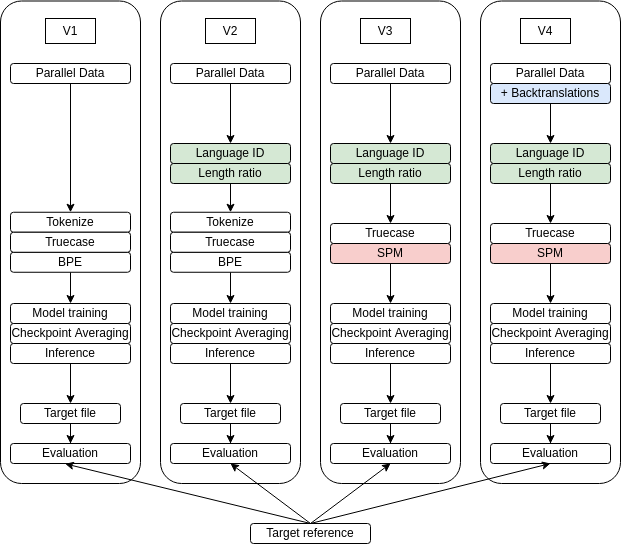
\includegraphics[width=10cm,keepaspectratio,height=10cm]{resources/pipeline.png}
\caption{Offline systems pipelines and versions.}\label{chap4:pipeline}
\end{figure}

\section{Results}

Table \ref{table:bleuoff} shows BLEU scores on WMT and CN evaluation sets for V0 through V3 systems.
With this system we did not achieve as good results as the ones our V0 system already had for the WMT tasks, while the performance for CERN News was not measured until we developed our V3 system, when CERN News was already compiled. 
For V2, we can see how the performance improved respect to V1, although we still did not reach the performance of the system that was already in production. 
Lastly, with V3 we achieved a similar performance as V0 for the WMT task, improving it in the case of wmt14 test set, and a significant improve in CERN News with respect to V0.

\begin{table}
\caption{En->Fr Bleu scores for WMT and CERN News evaluation sets.}
\centering
\begin{tabular}{l|c|c|c|c}\label{transformer:wmt:r}
System & WMT13 & WMT14 & CN21 & CN22 \\
\hline
V0 & \textbf{34.8} & 40.8 & 37.2 & 37.7\\
V1 & 32.1 & 39.1 & - & - \\
V2 & 32.6 & 39.4 & - & - \\
V3 & 34.0 & \textbf{41.0} & \textbf{38.3} & \textbf{38.7}\\
%v4 & 34.0 & 40.9 & \textbf{38.6} & \textbf{38.8}\\
%v3FTk100 & - & - & 42.0 & \textbf{43.1}\\
%v4FTk100 & - & - & \textbf{42.3} & 42.9\\
\end{tabular}
\label{table:bleuoff}
\end{table}


%307028269



\chapter{Domain Adaptation}\label{domad}
Given that we have knowledge of one of the use cases where our systems will be employed, we would be interested in increasing the performance in this specific context.
We have prior knowledge for certain characteristics of the sentences that our systems will be required to translate. We can leverage this fact to provide systems specialized on this domain.

For this task, since our systems depend on the data we make them available, we need resources of the specific domain to which we want to specialize. Often, data of one specific domain is scarcer than general data, as it is in the specific context of translating CERN documents that we address in our work. For this reason, instead of training a model only with data of the desired scenario, we perform \textit{domain adaptation} of general purpose systems. From a model that was fit to a general domain, we leverage smaller amounts of available in-domain data to modify its parameters so that it improves on the specific domain. 

In this chapter we present two techniques to perform domain adaptation, as well as the results of our systems when applied these techniques for our target domain. 

\section{Training with backtranslations}
As we saw in Section \ref{wordbased}, the use of monolingual data served to train the language model of the systems, the prior distribution $p(y)$ representing which sentences are more or less probable in a language. We saw too however that NMT approaches to the translation task model directly the distribution $p(y|x)$ (see Section \ref{nmtrnn}).
The technique of \textit{backtranslations} allows NMT models to make use of the information from monolingual resources. 

The idea of this technique is to use the monolingual resource as the target part of what would be a parallel corpus. Since the source part is missing, it will be generated through an automated process. We refer to this automatically generated data as the synthetic source, also known as backtranslations of the target sentences. In order to procure these automated translations, we use a MT model of reverse direction. If the target language of our system is French, we would use a system that has been trained to translate from French to English, and then generate the synthetic English source from our French monolingual resource. Once this parallel set is built, it would be added to the rest of the corpora that constitutes our training set, and a model would be trained from scratch. The method has shown to provide improved results in NMT systems by increasing the amount of data available \cite{DBLP:journals/corr/SennrichHB15a}.

\subsection{Experimental setup}\label{V4}
The use of backtranslations is not a technique thought as such for performing domain adaptation. In general, it allows the use of bigger amounts of data for NMT tasks, since we can leverage monolingual resources that are available, and it is widely used for this end \cite{DBLP:journals/corr/abs-1808-09381}. However, it is also the case in our in-domain scenario, that parallel data is scarcer and more difficult to gather than monolingual data. For this reason we make use of this technique with the aim of improving results on this target domain.

The in-domain data that we have available is sourced from the CERN Document Server\footnote{http://cdsweb.cern.ch/}. The site gathers different publications in the field of High Energy Physics, such as articles, books, reports, lectures, preprints, etc. From these, Apache Tika\footnote{https://tika.apache.org/} was used to extract the text from PDF files, constituting a corpora of 1.4 million sentences in French. These were later filtered with different techniques to increase the quality of the data.


%Monolingual \cite{sennrich-etal-2016-improving}
With the V4 system we continue the work developed in Chapter \ref{systems} for our offline systems. First of all we need to procure the English backtranslations for the French CDS corpus. In order to do so, we preprocess this data, truecasing the words and applying sentence piece to obtain a subword segmentation. Then, we use a trained MT model in the Fr->En direction to infer the translation of each sentence. At this point, we add this in-domain source to the total of sets that form our general-domain training data of Section \ref{dataset}, and build a new model following the same steps, techniques and parameter configurations as in our V3 system of Section \ref{V3}. We filter and preprocess the complete corpus of 310M sentences, configure and train the model for 1M updates, average the last 8 saved checkpoints, and perform the evaluation with our development and test sets. 
\subsection{Results}


Table \ref{table:bleuoffv4} shows BLEU scores on WMT and CN evaluation sets for V0, V3 and V4 systems.
We achieve small improvements in our CERN News evaluation sets, while the performance for the general domain did not decrease notoriously. The small changes on the results for this system could be a result of the reduced size of the CDS corpora in comparison to the size of the whole training set. We could still consider this model as a general purpose translation system, even if we have improved the results of our models for our specific target domain with domain-specific data.

\begin{table}
\caption{En->Fr Bleu scores for WMT, CERN and CERNnews evaluation sets (V4 backtranslations).}
\centering
\begin{tabular}{l|c|c|c|c}\label{transformer:wmt:r}
System & WMT13 & WMT14 & CN21 & CN22 \\
\hline
V0 & \textbf{34.8} & 40.8 & 37.2 & 37.7\\
V3 & 34.0 & \textbf{41.0} & 38.3 & 38.7\\
V4 & 34.0 & 40.9 & \textbf{38.6} & \textbf{38.8}\\
%v3FTk100 & - & - & 42.0 & \textbf{43.1}\\
%v4FTk100 & - & - & \textbf{42.3} & 42.9\\
\end{tabular}
\label{table:bleuoffv4}
\end{table}



\section{Finetuning}\label{fine}
In contrast to when we trained with backtranslations where a model was developed from scratch, finetuning works with small amounts of in-domain parallel data to adapt to the target domain. As starting point, it uses a model that has already finished its training. In our case, we adapt to the domain of physics at CERN a model previously trained for general purpose. Different finetuning techniques exist. Some of them modify the model for this adaptation process. For example, methods that add to the existing model extra \textit{adaptation layers} \cite{DBLP:journals/corr/abs-1803-10082} or those that \textit{freeze} certain parameters of the network while training the model for extra steps \cite{DBLP:journals/corr/abs-1801-06146}.

\subsection{Experimental setup}
The finetuning method that we will use keeps the architecture of the model without changes. Instead, we train the model for an small amount of extra steps, using exclusively a set of parallel data of the specific domain.
%Finetuning is with small amounts of data
%We keep the training of the model as it is.

Since finetuning requires smaller number of training steps by orders of magnitude, the time for adapting our models is considerably shorter as when training a model from the ground up. The process lasts hours instead of days or weeks. 
For this reason, we are able to develop 5 extra models parting from V3 Sentence Piece (see Section \ref{V3}). Four of these are built from CERN News training data (see Table \ref{CNTrain}), using the different sets that contain different percentages of the total CERN News training data according to their alignment quality of the sentences. The 5th model is built from the parallel text of CDS English backtranslations and the original sentences in French. 

For finetuning our models we also use Fairseq. Even if the preprocessing steps for the new training data remains the same, we vary some of the parameters of our trainer. We apply filtering, truecasing and sentence piece to the 5 different datasets. Then, we binarize each one of them separately with fairseq-preprocess in order to train 5 different experiments. We configure fairseq-train in the same way as described in V1 (see Section \ref{V1}), except for the lr-scheduler, which will be fixed. We use as value for the learning rate the value that the initial model had when its training finished. In addition, we modify to train for 5000 thousand steps, and keep checkpoints every 100 training updates. The training for the finetuning starts from the averaged checkpoint that was saved from V3 system after 1M of updates, and after the 5000 extra finetuing steps, we do not average checkpoints as we do when training a complete new model.
%even if recommend is to train with the last lr, we low it to have less agressive ft

\begin{figure}
\centering
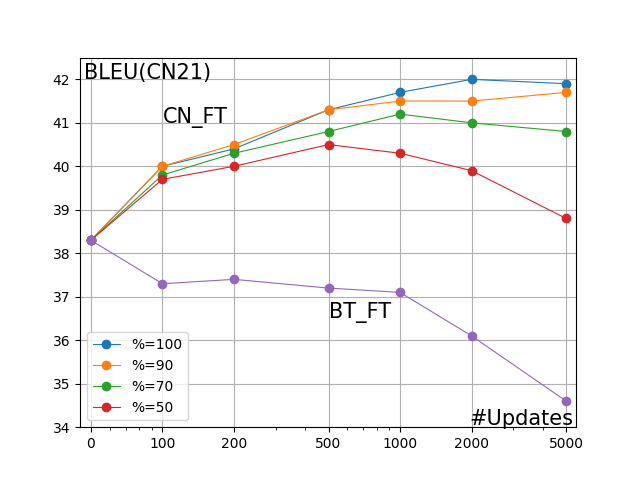
\includegraphics[width=10cm,keepaspectratio,height=10cm]{resources/CN21_bleu.png}
\caption{Results on CERN News development set for V4 finetuned on CDS backtranslations parallel set and on CERN News training set.}\label{pmid:cnft}
\end{figure}
\subsection{Results}

In Figure \ref{pmid:cnft},
plotting BLEU scores (y-axis) for our in-domain development set upon different number of updates (x-axis) corresponding to different checkpoints we can see how the performance for training with CERN News improves until a certain point and then starts to decrease. 
%This is a common behaviour on finetuning adaptations \cite{luong-manning-2015-stanford}. 
We observe the best result when training with 100\% of CERN News data and after 2000 training updates. This corresponds to a BLEU score of 42.0. In this configuration, the BLEU score for the CERN News test set was 43.1. These results constitute an improvement of 12.9\% in the development set and 14.3\% in the test set with respect to V0 X5gon.

After these results, we performed a second finetuning process with V4 with CERN News. Taking as starting point the final averaged checkpoint of our V4 system, we trained an extra model, using CERN News Training data. The best results of this finetuning were similar to the previous finetuning, with 42.3 and 42.9 BLEU scores for the CERN News development and test set respectively, as we can see in Table \ref{table:bleuft}. These were also achieved using 100\% of the CERN News training data.  



\begin{table}
\caption{Best results of En->Fr finetuned systems in BLEU scores for CERN News evaluation sets.}
\centering
\begin{tabular}{l|c|c}
System & CN21 & CN22 \\
\hline
V0 & 37.2 & 37.7\\
V3FTk100 & 42.0 & \textbf{43.1}\\
V4FTk100 & \textbf{42.3} & 42.9\\
\end{tabular}
\label{table:bleuft}
\end{table}




%Finetuning \cite{luong-manning-2015-stanford}



\chapter{Streaming NMT}\label{strnmt}
In this chapter we address a different kind of machine translation problems. In contrast to as explained in Section \ref{mt} and assumed in Chapter \ref{systems}, now we work with partial inputs at time of producing target translations, i.e. our systems start creating a translation before the complete source text is read.
%These are aimed to automate the task of simultaneous interpretation, where a speech is translated concurrently as it is produced \cite{ma-etal-2019-stacl}.

We consider two similar problems in this scenario, which we refer as \textit{simultaneous} and \textit{streaming} translation.
In simultaneous translation, we consider the case where we work on individual sentences. Systems produce target words sequentially with a certain delay as the input sentence is read. 
In streaming translation, the source is rather unbounded. We work with a stream of words, of unconstrained length, that is feed into the system for translation. This source is then translated similarly to simultaneous translation, producing target words with a time of delay with respect to the source words that have been read.
In this streaming setting, the past history of source and translated words can be leveraged as context to improve the quality of the systems \cite{https://doi.org/10.48550/arxiv.2203.02459}.

Since different components of a sentence are often differently structured among different languages (e.g. consider German or Japanese as subject-object-verb language versus subject-verb-object English) these \textit{online} systems are often required to produce a word before the corresponding source word has been read.
In general the online task is harder than the offline and with online systems a tradeoff is reached, between the quality of the translation that could optimally be produced in an offline system and the earliness in which the target text is available. 

We present in this chapter the online problem formally and describe a neural machine translation model for the task. We explain different measures of delay for these systems and describe a system developed for the simultaneous task. Finally, we  present results of this system on our development and test sets.

%Streaming \cite{https://doi.org/10.48550/arxiv.2203.02459}
\section{Formal setting}
As in Section \ref{mt}, we define the source $\vect{x}$ as a vector of $\vect{n}$ words, and the target as a vector $\vect{y}$ of $\vect{m}$ words. Since we are in an online scenario, we consider a function $g(t)$ which represents how many words of the source are available when the target word of position $t$ is produced. We refer to this function as the policy, and the way it is defined in a model will vary the behaviour of such system.

Now we consider the probability $p_g(\vect{y}|\vect{x})$ as the probability of $\vect{y}$ being a target translation of $\vect{x}$, taking into account that for the $t$'th target word, only the first $g(t)$ words of $\vect{x}$ are available to any method of translation. We are then interested in predicting the most probable target translation $\vect{y}_p$ of $\vect{x}$,
\begin{equation}\label{pg}
    \vect{y}_p = \arg \max_{\vect{y} \in Y} p_g(\vect{y}| \vect{x})
\end{equation}
where $Y$ is the set of possible sentences that can be produced in the target language.
Applying the product rule on the probability of each target word, we can rewrite the previous expression
\begin{equation}
    \vect{y}_p = \arg \max_{\vect{y} \in Y} \prod_{t} p_g(y_t | \vect{x}_{\leq g(t)}, \vect{y}_{<t})
\end{equation}
where we formalize our constraint on the available source and target words when producing the $t$'th word, $\vect{y}_{<t}$ being the previous words generated and $\vect{x}_{\leq g(t)}$ the first $g(x)$ source words. 

\section{Simultaneous Transformer model}
We adapt the Transformer for the streaming setting. In the following section we present the \textit{wait-k} policy and the \textit{multi-path-wait-k} model which is based on this policy.

\subsection{Wait-k policy}
Wait-k is a simple policy that is widely used in the simultaneous MT task.
The idea behind this policy is to produce target words always with a delay of k words with respect to the source. In this way, the first target word is produced when the system has available the first k source words. Upon this point, the system receives one more source word, and produces one more target word, in this way 1 writing operation after 1 reading operation, until all source words are read, and then the remaining of target words (if any) are produced.
If we had 
\begin{equation}
g(t) = t - 1, 
\end{equation}
this would mean that our system does not wait to produce the first word i.e. produces it without having seen any source word, and then the number of target words written would always surpass the number of source words read by one. This would be a wait-0 policy. Instead we have
\begin{equation}
g(t) = k + t - 1.
\end{equation}

In addition to this, we take into account that the length of the target usually differs from the source. We keep the idea that upon producing the target we are delaying the equivalent to k source words, thus we define the wait-k policy 
\begin{equation}\label{waitkgamma}
    g(t) = \left\lfloor k + \frac{t - 1}{\gamma}\right\rfloor 
\end{equation}
where we usually define the \textit{catchup} term $\gamma = |\vect{y}|/|\vect{x}|$ accounting for the source-to-target length ratio.


%Multipath \cite{DBLP:journals/corr/abs-2005-08595}
\subsection{Multi-path-wait-k model}\label{multik}
Following the wait-k policy, when producing word $y_t$, $g(t)$ source words would be available.
Training a model with a single k would imply that the value for this k has to be decided and fixed. This model could not fit well tasks where we require a different latency for translating other than the one that was used during training.

We follow the model described in \cite{DBLP:journals/corr/abs-2005-08595} where different values for k are used for training. In practice, we define a set of values, that as default range from 1 to $|\vect{x}|$. Then, for every different training batch, a value for k is randomly chosen from this set. This approximates the model
\begin{equation}
    E_K\left[ p_g(\vect{x} | \vect{y}, \vect{z}^k) \right] \approx \prod_{k\sim \mathcal{U}(K)} p_g(\vect{x} | \vect{y}, \vect{z}^k)
\end{equation}
where $p_g$ from (Eq. \ref{pg}) is conditioned on $\vect{z}^k$, the decoding path of reading source words and writing target words that the model would follow for a chosen a k.

In addition to this, this model is optimized with what we refer to as \textit{unidirectional encoding}. In the transformer architecture that we have thus far described, every time that an extra source word was available to the system the attention layers would need to be uptdated, so that representations of words take into account the new word. Instead of this, we use masked attention so that attention heads depend only of precedent words. In this way, attention is only computed once for the source, previous words not requiring an update when a new source token is available.

%Simultaneous \cite{ma-etal-2019-stacl}
%Slow Simultaneous \cite{DBLP:journals/corr/abs-1906-00048}

\section{Evaluation}
Since in simultaneous or streaming machine translation we reach a tradeoff between the quality and latency of our systems, we need metrics that measure this latency and that we can interpret. 
We will present results in 3 different measures of delay. These are Average Proportion \cite{ma-etal-2019-stacl}, Average Lagging \cite{DBLP:journals/corr/ChoE16}
and Differentiable Average Lagging \cite{DBLP:journals/corr/abs-1906-00048}. 

The timing information of these metrics is based on how many source words the system has read at each time $t$, when target word $y_t$ is produced. These metrics are thus independent of the environment and physical properties of the system. We do not rely on the information of the real time at which source words were produced.  

\subsection{Average Proportion}
Average Proportion computes simply the mean of the values of policy $g$ for each time $t$, when a target word is produced
\begin{equation}
    AP_g(\vect{x}, \vect{y}) = \frac{1}{|\vect{x}||\vect{y}|} \sum_{t=1}^{|y|}g(t).
\end{equation}
this mean is divided by $|x|$ so that the result is a value between 0 and 1.

We can find two flaws of average proportion that are discussed in the literature. First, since it is a metric between 0 and 1, it does not provide an easy readability on the number of words that the system is lagging. Second, it is sensitive on the length of the inputs. Following the example in \cite{DBLP:journals/corr/ChoE16}, if we consider a wait-1 policy and source and target of same length $|\vect{x}| = |\vect{y}| = 1$, $AP = 1$. If rather $|\vect{x}| = |\vect{y}| = 2$, $AP = 0.75$.
For smaller lengths, the metric is closer to 1. As lengths grow, average proportion tends to 0.5. Thus the metric penalizes long sentences, while the real delay of the system would not have changed. Average lagging is then proposed as a metric where these problems are not present.

\subsection{Average Lagging}
Average Lagging intends to account for how much our translation system is being delayed after a possible speaker that was being live translated. In this way, it compares the system policy $g$ with what would be an ideal wait-0 policy. For the case where $|\vect{x}|=|\vect{y}|$ we have
\begin{equation}
    AL_g(\vect{x},\vect{y}) = \frac{1}{\tau_g(|\vect{x}|)} \sum_{t=1}^{\tau_g(|\vect{x}|)} g(t) - (t-1)
\end{equation}
where the \textit{cut-off} step is defined as $\tau_g(|\vect{x}|) = \arg \min_t \left[g(t)=|x|\right]$. This is the first time $t$ where all source words are available, and then the rest of target words could be produced without further delay.
For this ideal case where $|\vect{x}|=|\vect{y}|$, with a wait-k policy, the metric has the property AL $ = k$.

In a more general case where $|\vect{x}|\neq|\vect{y}|$, in the same way that we adapted the wait-k policy to account for the source-to-target length ratio, we have 
\begin{equation}\label{al}
    AL_g(\vect{x},\vect{y}) = \frac{1}{\tau_g(|\vect{x}|)} \sum_{t=1}^{\tau_g(|\vect{x}|)} g(t) - \frac{(t-1) }{\gamma}
\end{equation}
where $\gamma = |\vect{y}|/|\vect{x}|$. In this case, for a system with a wait-k policy (Eq. \ref{waitkgamma}), the AL shows values that are aproximately k.

\subsection{Differentiable Average Lagging}
In \cite{DBLP:journals/corr/abs-1906-00048} where differentiable average lagging (DAL) is proposed, they try to adress the limitation that average lagging introduces when counting only up to the cut-off step $\tau$ in the computation of the average, which makes the metric non-diferentiable due to the argmin operation. They argue that this cut-off step is forced into the metric in order to keep the desired property of lagging $k$ with  a wait-k policy. Averaging for $|\vect{y}|$ instead of until $\tau$ would imply that the value $g(t)$ for $t > \tau$ would be kept constat at $g(t) = |\vect{x}|$ thus bringing the final average below $k$.

They propose that instead of bounding the average to $\tau$, writing operations should also contribute to the computation of the delay, not only reading operations. This follows the intuition that in a live translation, the words translated after the source sentence is completely available, do still take time to produce. First, $g'$ is defined  
\begin{equation}
    g'_d(t)=
    \begin{cases}
        g(t) &  t=1\\
        max\left[g(t),g'_d(t-1)+d\right] & t > 1 
    \end{cases}
\end{equation}
where d is the cost of a writing operation. The function $g'$ accounts for the time that has passed before the writing operation at time $t$. If $t=1$, no writing operations have been performed so far, thus $g'(t)=g(t)$. The second term of the max operation represents the time before the previous word was written plus the cost of writing such word, so we still account for a cost on time, even if no reading operations were performed since the writing of the previous word. Then, DAL is defined as
\begin{equation}
    DAL_d(\vect{x},\vect{y}) = \frac{1}{|\vect{y}|} \sum_{t=1}^{|\vect{y}|)} g'_d(t) - (t-1)d
\end{equation}
where the authors recommend defining $d = \frac{1}{\gamma} = \frac{|\vect{x}|}{|\vect{y}|}$, with which a very similar expression to AL (Eq. \ref{al}) is achieved:
%\begin{equation}
%    g'_d(t) = (t-1)d + \max_{1\leq i \leq t} \left[g(i) - (i - 1)d \right]
%\end{equation}
\begin{equation}
    DAL_{\frac{1}{\gamma}}(\vect{x},\vect{y}) = \frac{1}{|\vect{y}|} \sum_{t=1}^{|\vect{y}|)} g'_{\frac{1}{\gamma}}(t) - \frac{(t-1)}{\gamma}.
\end{equation}

In this way, reasoning about what should be considered delay in an online system, they achieve a metric that is differentiable and keep the idea in average lagging of measuring the delay against an ideal system or a live speaker.

\section{Experimental setup}
%\subsubsection{V4 multi-wath-wait-K}
In this section we explain the simultaneous model that we develop on this work. Implemented with fairseq (see Section \ref{fairseq}), we use the multi-path-wait-k model from Section \ref{multik} \cite{DBLP:journals/corr/abs-2005-08595}, trained with the same data and preprocessing that as for our offline V4 model described in Section \ref{V4}. Before all of this preprocessing, we preprocess the source part of the parallel data so that it mimics the output of an automatic speech recognition system. In this way, our system can be integrated in cascade to translate sources procedent from a live conference. The ASR preprocessed text, has a raw format, where for example all words are lowercased. The model learns then how to map from this type of text, to the target language in truecase. 

For training, resembling to the configuration in offline V4 (Section \ref{V4}), we use adam with $0.9$ and $0.98$ as beta values, inverse square root learning rate scheduler with 4000 warmup updates, dropout and label-smoothing of 0.1 and a batch size of 16000 pairs of sentences. The set of k values that the multi-k uses ranges from 1 to the maximum length of the sentences of our dataset. In the same way as for our offline systems, we perform checkpoint averaging with the last 8 training checkpoints,and train for 1M of updates.

We infer translations for our WMT and CERN News development sets with values for $k \in \{1,3,6,9,12,15\}$, and a catchup value of 1.25. 

\begin{figure}%
    \centering
    \subfloat[\centering]{{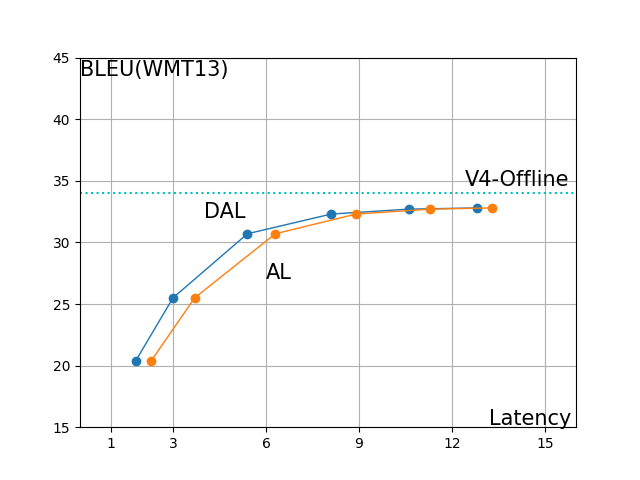
\includegraphics[width=7cm]{resources/onlineres.png} }}%
    \qquad
    \subfloat[\centering]{{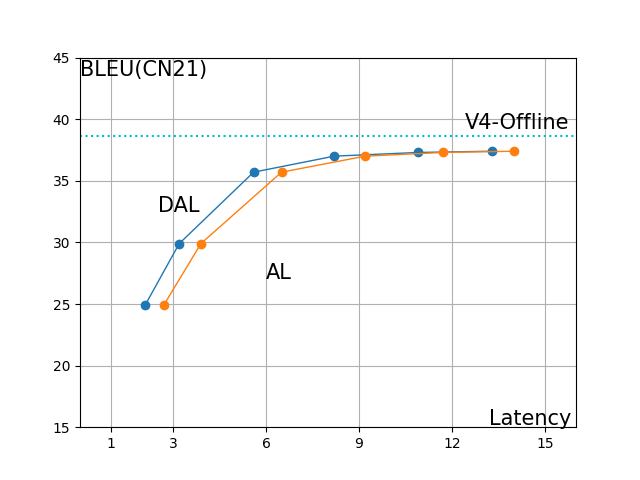
\includegraphics[width=7cm]{resources/onlineresCN.png} }}%
    \caption{(a) WMT13 Development set evaluation for different wait-k policies during inference time. (b) Same evaluation on CERN News 21 Development set. }%
    \label{chap6:onlineres}%
\end{figure}
\section{Results}
Results are presented for different online evaluation metrics combined with BLEU in Figures \ref{chap6:onlineres}.
%, appart from results in the AP metric, which are shown in Table \ref{table:apres}. 
We can see how upon augmenting the value of the delay $k$, the BLEU score grows until it stabilizes.
As expected, neither for WMT nor for CERN News, such high BLEU scores as those of which our offline systems offered (see Table \ref{table:bleuoff}) are reached, but they are traded by a short translating time. We compute BLEU and latency metrics on development and test sets in Table \ref{table:testres}, where we choose a wait-$k=6$ policy at inference time, which could be adapted depending on the required specifications of the system environment in which the model would be deployed. AL and DAL, highly correlated, show how the systems would be around 6 words behind a speaker being translated. Considering that French sentences tend to be larger than English ones in number of words, DAL could be paying the cost of numerous writing operations and thus consistently showing values greater than 6.


This system and our V4 offline system are ready to be deployed into the CERN infrastructure with little extra work. 
%\begin{figure}
%\centering
%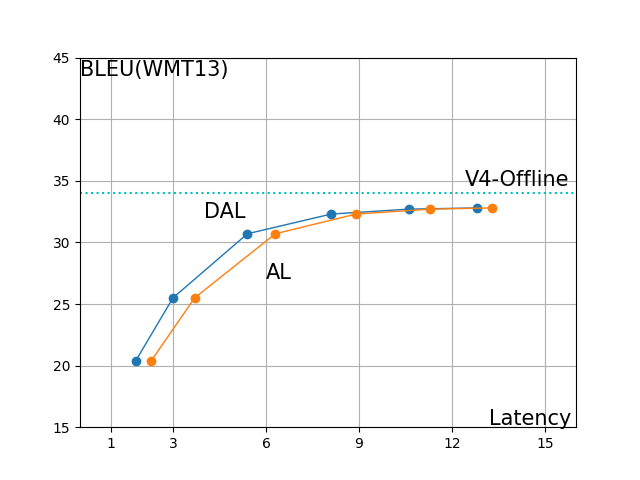
\includegraphics[width=10cm,keepaspectratio,height=10cm]{resources/onlineres.png}
%\caption{WMT13 Development set evaluation for different wait-k policies during inference time.}\label{chap6:onlineres}
%\end{figure}



\begin{table}
\caption{BLEU and latency results of our multi-path-wait-k system for development and test sets with a wait-6 policy at inference time.}
\centering
\begin{tabular}{l|c|c|c|c}
    Multi-k & WMT13 & WMT14 & CN21 & CN22 \\
\hline
    BLEU & 30.7 & 36.2 & 35.7 & 35.9 \\
    \hline
    AP & 0.8 & 0.7 & 0.7 & 0.7 \\
    AL & 5.4 & 5.5 & 5.6 & 5.5 \\
    DAL & 6.3 & 6.4 & 6.5 & 6.5 \\
\end{tabular}
\label{table:testres}
\end{table}





%In order to choose an adequate value of $k$ for, we would need to check the requirements on quality and latency for the specific task

%This means, sentences are lowercased 

%streaming can be adapted with a segmenter?
%ASR is solved task
%Ready to deploy

%defining in the following way



%%%%%%%%%%%%%%%%%%%%%%%%%%%%%%%%%%%%%%%%%%%%%%%%%%%%%%%%%%%%%%%%%%%%%%%%%%%%%%%
%                                 CONCLUSIONS                                 %
%%%%%%%%%%%%%%%%%%%%%%%%%%%%%%%%%%%%%%%%%%%%%%%%%%%%%%%%%%%%%%%%%%%%%%%%%%%%%%%

\chapter{Conclusions}\label{conclusion}

In this chapter we present a summary of the different tasks developed along the course of this work, as well as the different objectives achieved, difficulties found and lessons learnt. 

In Chapter \ref{intro} we presented the preliminary theoretical grounds in which the rest of our work settles.
We described ML in the AI field with statistical approaches to finally understand the more recent success of neural models. In parallel, we described the MT task from a non-neural point of view, after which we described NMT models up to studying in detail the current state of the art for NLP tasks Transformer model. We also learnt how evaluation of MT systems is crucial in their development, how this is usually performed and a way of interpreting these results.
In addition to this theoretical introduction, in this chapter we presented the objectives of our work, the structure and the framework in which it is carried out.

In Chapter \ref{dos} we centred our attention in data, as a fundamental part of MT systems. We presented the structure of MT parallel datasets, the challenges that entail gathering this data, and the sources that compose the principal sets that we used during the development of our models. Later, we moved to explain and compare different preprocessing and filtering techniques for MT, and which we applied to our data for developing our systems.

Chapter \ref{tres} was devoted to explain the compilation process and the content of the CERN News in-domain dataset. We explained all the steps that we applied, from crawling the online resources up to the final manual revision of the development and test sets.

In Chapter \ref{systems} we introduced Fairseq as the toolkit for developing our systems. We explained the preprocessing, training, inference and evaluation steps that compose the pipeline of our systems. Later, we described our experimental setup for the offline task, showing how we configured the models and which were the preprocessing steps for each version of our systems. Finally, we concluded with the results obtained, which were successfully compared against the production system of the MLLP research group to translate from English to French. The new system that was developed in this work was evaluated in terms of BLEU score and it achieved similar translation quality to the production system, but better results on the CERN News task.

Chapter \ref{domad} was dedicated to adapt our systems to the CERN domain. We presented training with backtranslations and finetuning as two different techniques for this purpose. The experimental setup for these techniques was described, explaining the training processes of our systems in each technique. Both techniques achieved improvements of our previous results. With CERN News finetuning a relative BLEU increase of 14.3\% 
with respect to the MLLP production system was achieved for CERN News task.

Lastly in Chapter \ref{strnmt} we moved to tackle the streaming NMT scenario. We described the problem formally, presenting afterwards the wait-k policy and the multi-path-wait-k model. Then, we showed three latency evaluation metrics, AP, AL and DAL. Finally, we presented a training of a multi-path-wait-k model implemented with Fairseq, and presented BLEU and latency results for WMT and CERN News task. 

As future work, the systems developed in this work, offline and streaming, will be deployed in a real production environment, and will be in this way integrated into the CERN infrastructure posibilitating the translation of their media videoconferences and internal resources. In addition, one inmediate next step following our work will be applying domain adaptation to online models. Furthermore, we can foresee the exploration of different finetuning techniques as those mentioned in Section \ref{fine}. We can also consider the idea of building a new in-domain corpus, with higher density of technical contents in physics, allowing us to adapt and evaluate our models to a greater extent in the domain of the CERN. 
\bibliographystyle{plain}
\bibliography{bibliography}

\cleardoublepage

%%%%%%%%%%%%%%%%%%%%%%%%%%%%%%%%%%%%%%%%%%%%%%%%%%%%%%%%%%%%%%%%%%%%%%%%%%%%%%%
%                           APÈNDIXS  (Si n'hi ha!)                           %
%%%%%%%%%%%%%%%%%%%%%%%%%%%%%%%%%%%%%%%%%%%%%%%%%%%%%%%%%%%%%%%%%%%%%%%%%%%%%%%

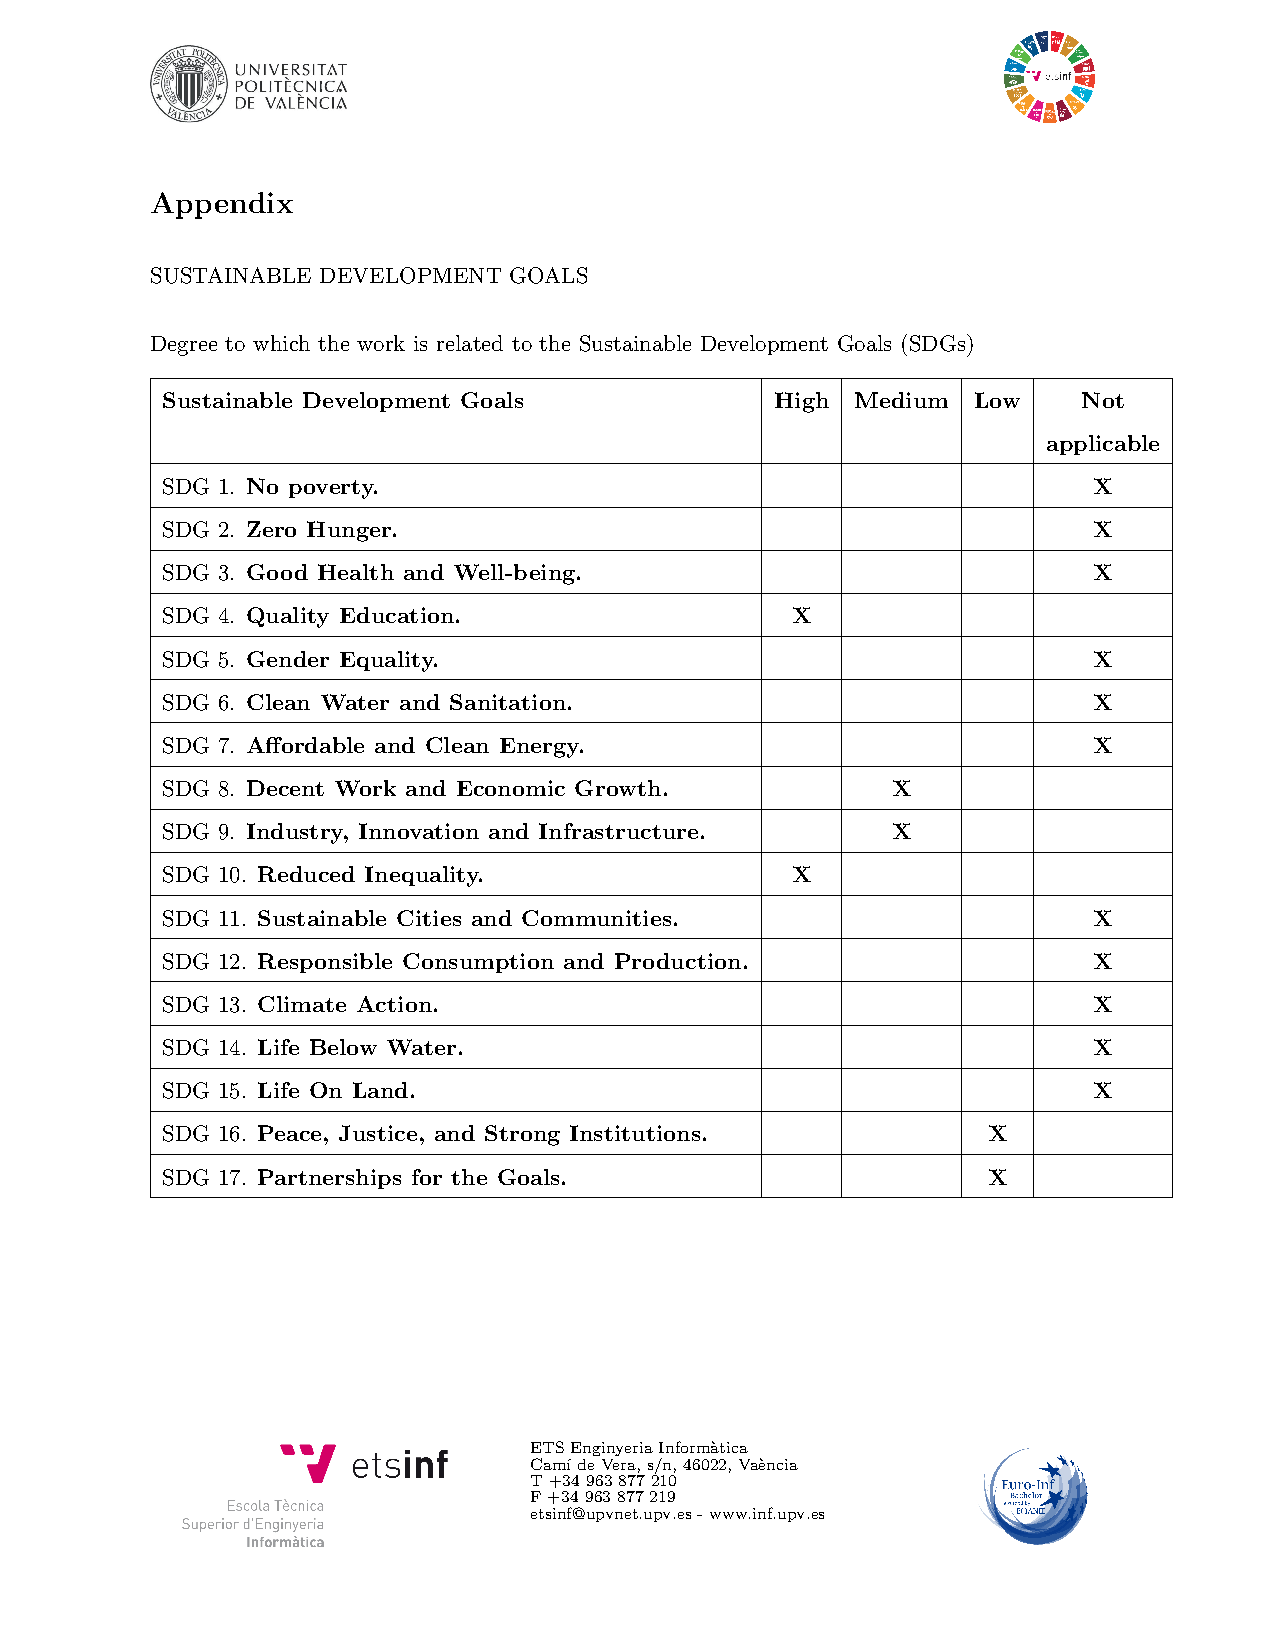
\includepdf[pages=-]{ods_etsinf_anexo.pdf}
%\APPENDIX

%%%%%%%%%%%%%%%%%%%%%%%%%%%%%%%%%%%%%%%%%%%%%%%%%%%%%%%%%%%%%%%%%%%%%%%%%%%%%%%
%                         LA CONFIGURACIO DEL SISTEMA                         %
%%%%%%%%%%%%%%%%%%%%%%%%%%%%%%%%%%%%%%%%%%%%%%%%%%%%%%%%%%%%%%%%%%%%%%%%%%%%%%%

%\chapter{Configuració del sistema}
%
%????? ????????????? ????????????? ????????????? ????????????? ?????????????
%
%\section{Fase d'inicialització}
%
%????? ????????????? ????????????? ????????????? ????????????? ?????????????
%
%\section{Identificació de dispositius}
%
%????? ????????????? ????????????? ????????????? ????????????? ?????????????
%
%%%%%%%%%%%%%%%%%%%%%%%%%%%%%%%%%%%%%%%%%%%%%%%%%%%%%%%%%%%%%%%%%%%%%%%%%%%%%%%%
%%                               ALTRES  APÈNDIXS                              %
%%%%%%%%%%%%%%%%%%%%%%%%%%%%%%%%%%%%%%%%%%%%%%%%%%%%%%%%%%%%%%%%%%%%%%%%%%%%%%%%
%


%%%%%%%%%%%%%%%%%%%%%%%%%%%%%%%%%%%%%%%%%%%%%%%%%%%%%%%%%%%%%%%%%%%%%%%%%%%%%%%
%                              FI DEL DOCUMENT                                %
%%%%%%%%%%%%%%%%%%%%%%%%%%%%%%%%%%%%%%%%%%%%%%%%%%%%%%%%%%%%%%%%%%%%%%%%%%%%%%%

\end{document}
